%Plantilla para escritura de memoria/tesis
%Universidad Técnica Federico Santa María, Santiago, ||fChile
%Departamento de Ingeniería Mecánica
%Ignacio Muñoz Quiroz
%Santiago, 11/06/2021

%--- DOCUMENT SETUP

\documentclass[12pt, oneside]{article} %Document definition class
\usepackage[utf8]{inputenc} %Indicates we are using ISO-8859-1(latin1)  o utf8
\usepackage[english]{babel}
\usepackage{graphicx}
\graphicspath{{Figures/}} % Location of the graphics files (set up for graphics to be in PDF format)
\usepackage[a4papper,left=3.0cm,right=2.5cm,top=3.7cm,bottom=2.5cm,includefoot]{geometry}
\usepackage{sectsty} %Resize section and subsection font size  
\sectionfont{\fontsize{25}{20}\selectfont}
\setlength{\parindent}{2em}
\setlength{\parskip}{1em}
\usepackage{setspace}



%--- LOAD PACKAGES
\usepackage{amsmath} % Math comands
\usepackage{amssymb} % Math symbols 
\usepackage{gensymb} % Physics symbols
%\usepackage{subfigure} % subfigures
\usepackage{caption}
\usepackage{subcaption} % subcaptions
%\usepackage{float} % complemento para figura
\usepackage{import} % Divide main.tex into separated file
%\usepackage{natbib} % Bibliography
%\usepackage{verbatim}  % Needed for the "comment" environment to make LaTeX comments
%\usepackage{hypcap} 
%\usepackage{pdfpages}
\usepackage{booktabs}
\usepackage{hyperref}
\usepackage{multirow}% Multirows for tables


\usepackage{array}% fix tab options on Tables
\newcolumntype{L}{>{\centering\arraybackslash}m{3.5cm}}

%--- 

%--- FRONT PAGE

\title{
    \begin{center}
    \vspace{-3.5cm}
    {\Large\textbf{UNIVERSIDAD TÉCNICA FEDERICO SANTA MARÍA}}\\
    \vspace{0.5cm}
    {\large DEPARTAMENTO DE INGENIERÍA MECÁNICA}\\
    {\large SANTIAGO, CHILE}\\
    \vspace{0.5cm}
    
    
\includegraphics[scale=0.55]{Logo_UTFSM.png}

    \vspace{0.25cm}

    {\Large ESTUDIO DEL COMPORTAMIENTO CINÉTICO Y TERMODINÁMICO DE LLENADO DE NANOTUBOS ESTRECHOS DE CARBONO SUJETOS A CAMPOS ELÉCTRICOS, A TRAVÉS DE SIMULACIONES DE DINÁMICA MOLECULAR CLÁSICA}
    
    \vspace{1cm}
    
    {\large \textbf{IGNACIO TOMÁS MUÑOZ QUIROZ}}\\
    \vspace{0.35cm}
    {\normalsize MEMORIA PARA OPTAR AL TÍTULO DE INGENIERO CIVIL MECÁNICO}\\
    
    \vspace{0.5cm}
    
    {\normalsize Profesor Guía: PhD. Christopher Cooper}\\
    {\normalsize Profesor  Coreferente: PhD. Harvey A. Zambrano}\\
    {\normalsize Profesor  Coreferente: PhD. José Antonio Gárate}\\
    \vspace{0.3cm}
    {\normalsize \textbf{MES - AÑO}}
    \end{center}
}
\author{} % Left blank
\date{} % Left blank
%--- 

%--- PAGE SETUP
\usepackage{fancyhdr}
\pagestyle{fancy}
\fancyhead{}
\fancyfoot{}
\rfoot{\thepage}
\rhead{\leftmark}
%\renewcommand{\headrulewidth}{0pt}


%---

%--- DOCUMENT CORE

\begin{document}

\pagestyle{empty}
\pagenumbering{roman} % Add roman numbers for first pages
\setcounter{page}{0}
\maketitle %Add title page 

\renewcommand{\baselinestretch}{2}
\setstretch{1.2}

\section*{Abstract}
%\vspace{2cm}
The free energy of solvation $\Delta G^{solv}$ is the energy associated with the process of reorganizing solvent molecules, like water, around a solvated molecule, i.e, the proccess of moving the solute from vaccum  to it's position into the solvent. This process will be thermodynamically favorable only if the overall Gibbs energy of the solution is decreased, compared to the Gibbs energy of the separated solvent and solute. It's also function as an indicator of how probable will be a molecular system, in terms of its configuration, compare to others. 
%This is extremely useful in drug design industries because provides a tool to forecast, throw computer simulations, different versions of synthetic molecules before the manufacture process. 

$\Delta G^{solv}$ can be separated in two components: $\Delta G_{polar}$ and $\Delta G_{non-polar}$. The first is define as the  free  energy  of  creating  the  solute’s  charge  distribution  inside  a pre-existing solute cavity, and the second term, correspond to work required to place an uncharged solute insidethe solvent and generates a dry cavity on it. 

In this work, Molecular Dynamics technique (explicit model) was perform using GROMOS simulation software to calculate the van der Waals $\Delta G_{vdw}$ cavity-formation free energy for 20 alanine peptides divided in extended and helix configurations, ranging from 1 to 10, and compare the results with two impliri solvent models models: the standard model based on the molecular surface of the solute, and a new methodology which has a closer physical meaning modeling the solute as an uncharged capacitor.

An extended overview of the MD method is provided with the methodology for implementing GROMOS simulation software not just to replicate these results, but also for the calculation of the relative free energies of any structure or compound of interest. 
\section*{Resumen}
La energía libre de solvatación $\Delta G^{solv}$ es la energía asociada al proceso de reorganización de las moléculas de disolvente y soluto, en moléculas solvatadas. Este proceso es termodinámicamente favorable solo si la energía libre de Gibbs de la solución es menor, comparada con la energía libre de Gibbs de solvente y molécula por separado. Este parámetro también funciona como un indicador de qué tan probable podría ser una configuración de un sistema molecular, en comparación a otros. 

$\Delta G^{solv}$ puede separarse en dos componentes: $\Delta G_{polar}$ y $\Delta G_{no-polar}$. El primer término se define como la energía libre necesaria para crear la distribución de cargas del soluto en una cavidad pre-existente, y el segundo término corresponde al trabajo requerido para ubicar una molécula de soluto no-cargado en el solvente generando una cavidad seca en este último. 

En este trabajo, se usó la técnica de Dinámica Molecular junto al software de simulación GROMOS para calcular la energía libre de vand der Waals $\Delta G_{vdw}$ necesaria para generar la cavidad para 20 péptidos de alanina divididos en dos tipos de estructuras: hélice y extendida, cuya composición va desde 1 a 10 monómeros. Los resultados fueron contrastados con dos modelos: modelos implíticos tradicionales, y una nueva metodología que tiene una fundación más profunda y un significado físico más cercano a la realidad.
Se presneta también una descripción general de la matodología MD junto con el flujo de información usado por el software GROMOS, no solo para replicar los resutlados de este trabajo, sino que también apra el cálculo de energías libres de cualquier estrucutra molecular de interés. 









\newpage

\tableofcontents
\newpage
\listoftables
\newpage
\listoffigures
\newpage
\section*{Acronymus}

\begin{table}[th]
    \centering
    \begin{tabular}{l|l}
    \toprule
         Acronym &  Definition\\
         \midrule
         CM & Classical mechanics\\
         GROMOS & GROningen MOlecular Simulation\\
         MC & Monte Carlo\\
         MD & Molecular dynamics\\
         PDB & Protein Data Bank\\
         QM & Quantum mechanics\\
         SASA & Solvent-Accessible Surface Area\\
         TI & Thermodynamic Integration\\
         VMD & Visual Molecular Dynamics\\
         Z & Atomic number\\
         \bottomrule
    \end{tabular}
    \caption{Acronyms used in the text and their definitions.}
    \label{tab:acronymus}
\end{table}

\pagestyle{plain}
\pagenumbering{arabic}

\renewcommand{\baselinestretch}{2}
\setstretch{1.2}

\section*{Abstract}
%\vspace{2cm}
The free energy of solvation $\Delta G^{solv}$ is the energy associated with the process of reorganizing solvent molecules, like water, around a solvated molecule, i.e, the proccess of moving the solute from vaccum  to it's position into the solvent. This process will be thermodynamically favorable only if the overall Gibbs energy of the solution is decreased, compared to the Gibbs energy of the separated solvent and solute. It's also function as an indicator of how probable will be a molecular system, in terms of its configuration, compare to others. 
%This is extremely useful in drug design industries because provides a tool to forecast, throw computer simulations, different versions of synthetic molecules before the manufacture process. 

$\Delta G^{solv}$ can be separated in two components: $\Delta G_{polar}$ and $\Delta G_{non-polar}$. The first is define as the  free  energy  of  creating  the  solute’s  charge  distribution  inside  a pre-existing solute cavity, and the second term, correspond to work required to place an uncharged solute insidethe solvent and generates a dry cavity on it. 

In this work, Molecular Dynamics technique (explicit model) was perform using GROMOS simulation software to calculate the van der Waals $\Delta G_{vdw}$ cavity-formation free energy for 20 alanine peptides divided in extended and helix configurations, ranging from 1 to 10, and compare the results with two impliri solvent models models: the standard model based on the molecular surface of the solute, and a new methodology which has a closer physical meaning modeling the solute as an uncharged capacitor.

An extended overview of the MD method is provided with the methodology for implementing GROMOS simulation software not just to replicate these results, but also for the calculation of the relative free energies of any structure or compound of interest. 
\section*{Resumen}
La energía libre de solvatación $\Delta G^{solv}$ es la energía asociada al proceso de reorganización de las moléculas de disolvente y soluto, en moléculas solvatadas. Este proceso es termodinámicamente favorable solo si la energía libre de Gibbs de la solución es menor, comparada con la energía libre de Gibbs de solvente y molécula por separado. Este parámetro también funciona como un indicador de qué tan probable podría ser una configuración de un sistema molecular, en comparación a otros. 

$\Delta G^{solv}$ puede separarse en dos componentes: $\Delta G_{polar}$ y $\Delta G_{no-polar}$. El primer término se define como la energía libre necesaria para crear la distribución de cargas del soluto en una cavidad pre-existente, y el segundo término corresponde al trabajo requerido para ubicar una molécula de soluto no-cargado en el solvente generando una cavidad seca en este último. 

En este trabajo, se usó la técnica de Dinámica Molecular junto al software de simulación GROMOS para calcular la energía libre de vand der Waals $\Delta G_{vdw}$ necesaria para generar la cavidad para 20 péptidos de alanina divididos en dos tipos de estructuras: hélice y extendida, cuya composición va desde 1 a 10 monómeros. Los resultados fueron contrastados con dos modelos: modelos implíticos tradicionales, y una nueva metodología que tiene una fundación más profunda y un significado físico más cercano a la realidad.
Se presneta también una descripción general de la matodología MD junto con el flujo de información usado por el software GROMOS, no solo para replicar los resutlados de este trabajo, sino que también apra el cálculo de energías libres de cualquier estrucutra molecular de interés. 








\setcounter{section}{0}
\section{Introduction}\label{sec:intro}


\vspace{3cm}
\par

\subsection{Life is based on chemical interactions}

Understanding the basis of any biological phenomena is inseparable from understanding the principles that govern the behavior of atoms and molecules. All biological functions depend on events that occur at the molecular level. These events are directed, modulated, or detected by complex biological machines, which are themselves large molecules or clusters of molecules. Included are proteins, nucleic acids, carbohydrates, lipids, and complexes of them. Many areas of biological science focus on the signals detected by these machines or the output from these machines.

Most of biological processes happens in solution, mostly water, with tightly regulated concentrations of ions such as sodium and chloride. These solvent molecules strongly influence the structure and function of molecules, affecting protein folding and stability, as well as the affinity and specificity with which bio-molecules bind.

%As engineers, 
\par








\subsection{Molecular Structure}\label{subsec:molecular_structure}

As we know, molecules are composed of atoms, which are the units of matter that correspond to the elements in the periodic table. For example, only a few of these elements are abundant in cells. In fact, the vast majority of biological matter, about 99\% is made of just six elements: carbon, hydrogen, nitrogen, oxygen, sulfur, and phosphorus \cite{museums1992introduction}. Molecules such as proteins, carbohydrates, lipids, and nucleic acids, are made out of carbon as it's main backbone.\par

Atoms, in turn, are composed of particles known as protons, neutrons, and electrons. The properties of each particle is shown in Table \ref{table:massandcharge}. Protons and neutrons reside in the atomic nucleus and account for almost all of the mass of the atom. The number of protons present in an atom’s nucleus, its atomic number (Z), determines the identity of that atom as an element. 

\par\par

\begin{table}[th] %th for exact position.
    \centering
    \begin{tabular}{l|c|c|c|c}
    \toprule
    Particle            &   Mass [kg]       &   Relative mass [amu] &   Charge [Coulomb]    &   Charge\\
    \midrule
    Proton ($p^{+}$)      &   $1.6726x10^{-27}$ &   1.007                &   $1.6022x10^{-19}$     &   +1\\
    Neutron (n)         &   $1.6749x10^{-27}$ &   1.008                  &   0                   &   0\\
    Electron ($e^{-}$)    &   $9.1094x10^{-31}$ &   $5.489x10^{-4}$       &   $1.6022x10^{-19}$     &   -1\\
    \bottomrule
    \end{tabular}
    \caption{Mass and Charge of individual protons, neutrons and electrons.}
    \label{table:massandcharge}
\end{table}     

\subsubsection{Atomic Structure: Bohr's Model}

Presented by Niels Bohr and Ernest Rutherford in 1913, the Bohr's Model offers a representation of how electrons orbits around the nucleus of an atom. The electron orbits into shells:  The first shell contains 2 electrons, while the next shell can hold 8 electrons. The arrangement of electrons around the atomic nucleus is complex, and electrons do not simply orbit the nucleus as a planet would orbit a star. Broadly speaking, electrons are located in concentric shells that surround the nucleus. The shells that are closer to the nucleus are generally lower in energy than the shells that are farther from the nucleus, meaning that placing an electron in a shell that is closer to the nucleus is more stable and more favorable than placing an electron in a shell that is farther from the nucleus. Because of this, electrons fill shells from the inside to the outside. Electrons in atoms with few electrons are in shells close to the nucleus, whereas atoms with many electrons first utilize the shells that are closer to the nucleus and then those that are farther from the nucleus once the inner shells are filled. 

\subsubsection{Atomic Structure: Quantum Mechanics}

Electrons don't travel in neat 2D circular orbits as the Bohr's model suggest, in fact we can't even determine the position and the velocity of an electron. Instead, we can make predictions about electron's general locations in 3D space. These regions that we call \textbf{orbitals} are the locations in space that has about 90\% certainty that an electron is located somewhere within that region \cite{brown2016introduction}. In Figure \ref{fig:orbitals} are represented the shapes that orbitals can take around the atom. Each orbital now can hold two electrons. In the case of carbon, we focus on the \textit{"s"} orbital, which are spherical in shape with the nucleus of the atom at the center, and \textit{"p"} orbital, which have the shape of the number eight, or the infinity symbol with the nucleus also at the center. 

\begin{figure}[h]
    \centering
    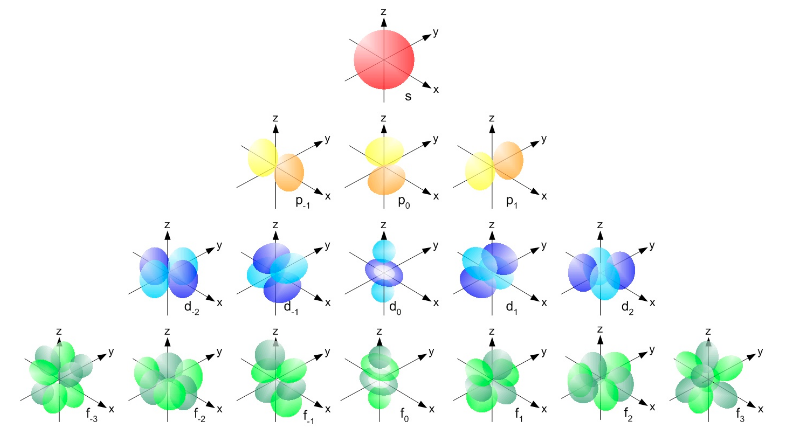
\includegraphics[scale=0.5]{Figures/Chapter1/orbitals.png}
    \caption{Schematics showing the general shapes of s, p, d, and f orbitals.}
    \label{fig:orbitals}
\end{figure}

In the ground state, electrons will occupy the lowest energy orbitals first. In the case of the element \textbf{carbon}, which contains 6 electrons on it's outer shell, the first orbital that fill is the \(1s\), which an hold 2 electrons. Next, is the \(2s\)-orbital which is a larger sphere, and can also hold 2 electrons. Finally, we have \(3p\)-orbital: each one aligned along the \(x,y\) and \(z\)-axis , each capable of 2 electrons so they are filled with one electron in the \(px\)-orbital and one in the \(py\)-orbital. To be stable, carbon wants to fill these three p orbitals with 2 electron each. 

The interaction between different atom's orbitals results in ``connections" between them and can be thinking of forces of attraction (or in some cases repulsion). There are two types of interactions: \textbf{bonded} and \textbf{non-bonded} interactions. The first is know as  chemical bonds, and there are three types: (1) \textit{Ionic bond}, formed when one atom donates valence electrons to another atom. (2) \textit{Covalent bond}, when both atoms share pairs of valence electrons, and (3) \textit{Metallic bond}, formed between a cloud of free electrons and the positively charges ions in a metal. interact. For example, a water molecule is made of one oxygen atom connected to two hydrogen atoms through single covalent bonds.  However, some covalent bonds involve the sharing of more than one pair of electrons between atoms.  Double and triple bonds involve the sharing of four and six valence  electrons,  respectively.   This  versatility  allows  carbon  to  create  many  different kinds of molecules which gives this particular element, a vast number of properties. 

The second interaction, \textbf{non bonded}, is explain in detail in Section \ref{subsec:FF} because is the main objective of this work. Study the behavior of a particular component of this type of interaction. 


\subsection{Computer Simulation of Molecular Systems}\label{subsec:computation}

The role of computation in biology, biological chemistry, and biophysics has shown a steady increase over the past few decades. The continuing growth of computing power (in particular in the context of personal computers) has made it possible to analyze, compare, and characterize large and complex data sets that are obtained from experiments on bio-molecular systems. \cite{van2006biomolecular}. Chemical systems are generally too complex to be treated by analytical theoretical methods so it becomes a necessity to implement numerical analysis to study and predict some properties and configurations.

Computer simulations on models of physical systems have been carried out for more than 65 years now \cite{oostenbrink2007applications}. Many developments have turned molecular dynamics simulations into a valuable tool, complementary to experimental investigation, to probe into structure, dynamics, and activity of large biologically relevant molecules. The thermodynamic information that can be obtained from computer simulations allows analysis and understanding of molecular processes and prediction of molecular properties, highly valued information in medical chemistry and drug design. 




\subsection{Objectives}
\begin{itemize}
    \item The main objective of this work, is to calculate the free energy of solvation (non-polar) of 20 peptides using classical Molecular Dynamics Simulation method.
    \item Compare the results of the explicit MD model with the calculations given by the implicit solvent models available by measure the accuracy of them.
    \item  Become familiar with the use of GROMOS++ software for the calculation of free energies using Thermodynamic Integration. 
    \item Study the behavior of the van der Waals interaction and its contribution to the solvation process. 
    \item Simulate 20 alanine-peptides in a pre-equilibrated water box to preform the free energy calculations. 
\end{itemize}

This document is organized as follow: Section \ref{sec:MD}, presents an overview of the Molecular Dynamics (MD) method, which is the tool to preform the calculations of the free energies of solvation described in the abstract and the criteria and requirements needed to build this method. It also provides a characterization of the force-fields whit a special attention to describe the nature of non-bonded interaction which is the main subject treated in this work.
In Section \ref{sec:implicit}, implicit solvent models are explain with they advantages and disadvantages and also the reasons to use this methods as an alternative to MD. In particular, Section \ref{subsec:CC_method} described a novel way to calculate $\Delta G_{solv}$, sharing the same ideas as the implicit solvent models, but with a clearer physical meaning than current available models. 
Next, Section \ref{sec:Free_energy} presents the underlying thermodynamic and statistical mechanics theory that had been develop to calculate free energies, with the mathematical construction of these models. Section \ref{sec:methods} talks about the methodology used to compute the free energy results, starting with the preparation of the molecular structures (Section \ref{subsec:strucutre_prep}), following by a review of the scope and functionality of GROMOS simulation software, explaining how it was used to preform such calculations step by step. 
Finally, in Section \ref{sec:results} the results and comparison between the models explained above are presented.


\section{Molecular Dynamics}\label{sec:MD}

\vspace{3cm}
\par

Computation based on molecular models is playing an increasingly important role in biology, biological chemistry, and biophysics. Since only a very limited number of properties of bio-molecular systems is actually accessible to measurement by experimental means, computer simulation can complement experiment by providing not only averages, but also distributions and time series of any definable quantity, for example, conformational distributions or interactions between parts of systems. As it's mentioned in section \ref{subsec:computation}, computer modeling of bio-molecular systems has become a standard technique to study and describe the properties and behaviour of such systems in terms of interactions between atoms or electrons of atoms.

Molecular dynamics (MD) is a \textbf{computer simulation method} for analyzing the physical movements of atoms and molecules. The atoms and molecules are allowed to interact for a fixed period of time, giving a view of the dynamic ``evolution" of the system. Computer simulations can then be used to test and validate theories and models or to replicate and compare experimental results.

There are some key elements that must be taken into account when developing any simulation exercise. The model approximations must be consider to ensure applicability to the system of interest, and appropriate statistical analyses must be performed (for which sufficient sampling is required).

In general, to set-up a particle based simulations, there are four main choices to consider for the model that will be used which will be discussed in the next four sections as it's shown in Figure \ref{fig:md_cicle}: The degrees of freedom to be considered, interactions that occur between the chosen degrees of freedom, how they are to be sampled, and how the boundaries and/or external forces of the system are to be considered \cite{van2006biomolecular}. 
\begin{figure}[h]
    \centering
    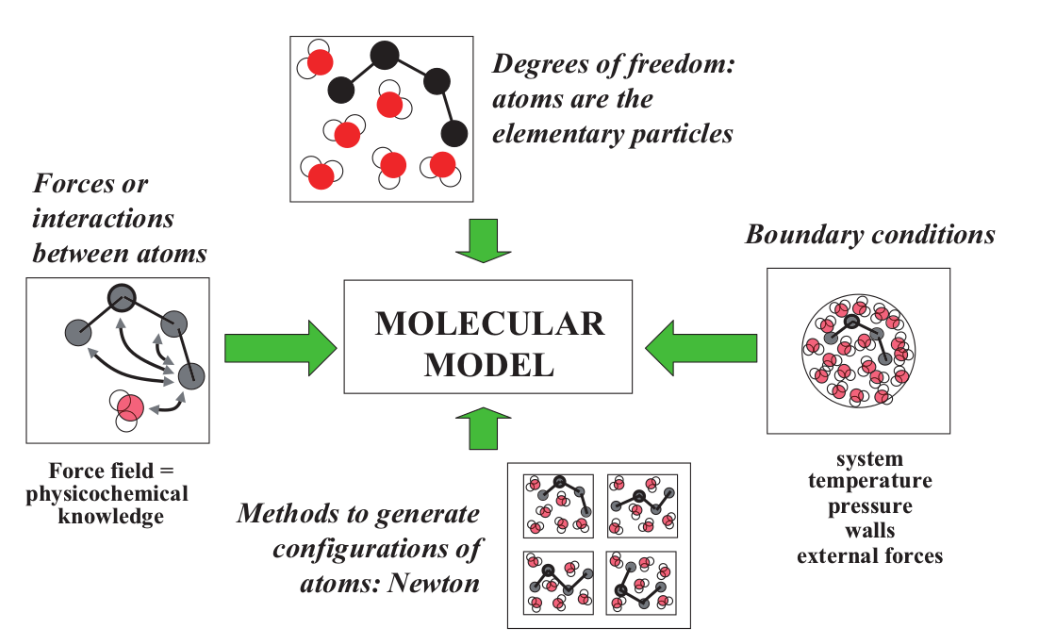
\includegraphics[scale=0.4]{Figures/Chapter2/MD_cicle.png}
    \caption{Four basic choices in the definition of a model for molecular simulation. Figure from Van Gunsteren et al. \cite{van2006biomolecular}}
    \label{fig:md_cicle}
\end{figure}

\subsection{Degrees of freedom}\label{subsec:degrees}

This criteria is oriented to determine which molecular description are explicitly considered in the model and is strictly related to the resolution of the system of interest. The level of modeling chosen to describe a particular bio-molecular process depends on the type of process. This will determine the theory employed, ranging from quantum to classical mechanics. In this particular case of study, we are interest on evaluate the interaction between the solvent and the solute which is driven by weak, non-bonded inter-atomic interactions. Therefore, these processes are most promisingly modeled at the atomic or molecular level. In Table \ref{tab:Degree} are organized by level of detail, the methods for different molecular descriptions. 

\begin{table}[h]
    \centering
    \begin{tabular}{L|L|>{\centering\arraybackslash}p{4.5cm}|p{3cm}}
    \toprule
        Methods & Degrees of freedom & Properties, processes & Time scale \\
    \midrule
        quantum dynamics & atoms, nuclei, electrons & excited states, relaxation, reaction dynamics & picoseconds \\
        
        quantum mechanics & atoms, nuclei, electrons & ground and excited states, reaction mechanisms & no time scale \\
        
        classical statistical mechanics (MD, MC, force fields) & atoms, solvent & ensembles, averages, system properties, folding & nanoseconds \\
        
        statistical methods (database analysis) & groups of atoms, amino acid residues, bases & structural homology and similarity & no time scale \\
        
        continuum methods (hydrodynamics and electrostatics) & electrical continuum, velocity continuum etc. & rheological properties & supramolecular \\
        
        kinetic equations & populations of species & population dynamics,  signal transduction & macroscopic\\ 
    \bottomrule
        
    \end{tabular}
    \caption{Examples of levels of modeling in computational biochemistry and molecular biology. Table from from Van Gunsteren et al. \cite{van2006biomolecular}}
    \label{tab:Degree}
\end{table}

As it is shown in Table \ref{tab:Degree}, the models were categorized by order of approximation, ranging from quantum descriptions in the form of quantum mechanics (QM) based models which take into account the interaction between atom's orbitals as is described in Section \ref{subsec:molecular_structure} with multiple degrees of freedom, to approximations for heavy and slow particles on a larger scale were the processes involved are very well described by classical mechanics. The cost of the energy and force evaluation is primarily determined by two factors: the degrees of freedom that are considered and the functional form of the Hamiltonian (Section \ref{subsec:FF}). One can move from a quantum-mechanical description of the system where the electronic degrees of freedom are modeled explicitly, to a classical description where one atom is treated as one particle, to a coarse-grained description where groups of atoms are merged into one particle. A reduction in the number of degrees of freedom can, however, also be obtained by reducing the system size or treating parts of the system (e.g., the solvent) as a continuum \cite{christ2010basic}.

The choice of which degrees of freedom are modeled explicitly depends on the system of interest and the property one wishes to estimate. If a certain degree of freedom is believed to have no effect on the property of interest, it can be omitted and the computing time gained invested in sampling the relevant degrees of freedom more extensively.
\subsection{Potential Energy Function: The Force Field}\label{subsec:FF}

A bio-molecular force field generally consists of potential energy terms representing covalent interactions between atoms (such as bond-stretching, bond-angle bending, improper and proper dihedral-angle torsion), and non-bonded interactions between atoms in different molecules and between atoms in a molecule that are separated by more than two or three covalent bonds \cite{van2006biomolecular}. Consider a system that contains $N$ particles that are treated explicitly in the model. Often, these particles are atoms, but also groups of atoms can be treated as a single particle, such as hydrocarbons  like $CH , CH_{2} , CH_{4}$ groups. In classical simulations, the system is fully defined by the positions $\textbf{``q"}$, and the conjugate momenta, $\textbf{``p"}$, of the individual particles, where $r$ and $p$ represent 3-N dimensional vectors. In this work, we will use $q_{i}$ and $p_{i}$ for the three-dimensional vectors describing the position and momentum of the particle $``i"$. The potential energy function that determine the system, the \textbf{Hamiltonian}, is written as:
\begin{equation}
    H(p,q)= K(p)+V(q)
    \label{eq:hamiltonian}
\end{equation}
where $K(p)$ is the kinetic energy which can be
\begin{equation}
    K(p,m)=\sum_{i=1}^{N} \frac{p_{i}^{2}}{2m_{i}} = \sum_{i=1}^{N} \frac{1}{2}m_{i}v_{i}^{2}
\end{equation}
$V(r)$ in equation \ref{eq:hamiltonian} is the potential energy, describing the interaction between the particles in the system and possibly external influences on the system. It's a function of the particle position $\textbf{``q"}$. The functional form and parameters describing $V(r)$ is called \textbf{force field}. There are several well-known force fields for biomolecular simulation described in the literature, such as AMBER \cite{amber}, CHARMM \cite{charmm}, ECEPP/3 \cite{ECEPP/3}, and GROMOS \cite{van2005gromacs}\cite{gromos1}, and it takes different forms depending on the description of the system, and is usually a sum of multiple potential energy terms which describe different contributions corresponding to physical (or special) interactions. The potential energy is usually written as a sum over different contributions, separated in physical interactions and any special (unphysical, such as distance restraints between atoms and positional restrains) interaction one might want to apply to the system
\begin{equation}
    V(q)=V^{phys}(q) + V^{special}(q)
    \label{eq:v_general}
\end{equation}
The first term of Equation \ref{eq:v_general} is the mathematical description of the sum of various terms describing the bonded (bon) and nonbonded (nonb) interactions between particles. Bonded potential energy can be divided further to account for bonds, bond angles, harmonic (improper) dihedral angles and torsional or proper dihedral angles (Equation \ref{eq:bond_inter}), and not bonded interaction are are the sum of electrostatic (Coulomb) and van der Waals (Lennard-Jones potential) interactions between pairs of atoms (Equation \ref{eq:nonb_inter}).
\begin{equation}
    V^{bon}(q)= V^{bond}(q)+ V^{angle}(q)+ V^{imp}(q)+ V^{tor}(q)
    \label{eq:bond_inter}
\end{equation}
\begin{equation}
     V^{nonb}(q)=  V^{vdw}(q)+ V^{elec}(q)
     \label{eq:nonb_inter}
\end{equation}

\subsubsection{Force-Field Bonded Interactions}

In the followin sections, $V^{bon}$ terms are explain according to the GROMOS force field which is use in this work.

\subsubsection*{Bond stretching force-field term}
The potential energy term associated with bond-stretching interactions is the term $V^{bond}(q)$ in Equation \ref{eq:bond_inter} and it's the function describing the potential energy associated with the stretching of a single bond and has the form of an harmonic oscillator given by:
\begin{equation}
    V^{bond}(q) = \sum_{n=1}^{N}\frac{1}{2}k_{b}{(b_{n}-b_{n}^{0})}^2
    \label{eq:pot_bond}
\end{equation}
where the quantities $k_{b}$ and $b_{n}$ represent force-field parameters, force constant and reference length, respectively, characteristic for the specific bond n, and $N$ the total number of covalent bonds. 


\subsubsection*{Bond-angle bending force-field term}
The potential energy term associated with bond angle bending interactions is the term $V^{angle}(q)$ in Equation \ref{eq:bond_inter}. Each definable covalent bond angle associated with one and only one bending term in the GROMOS force and this term represent the function describing the potential energy associated with the bending of a single bond angle. It's given by: 
\begin{equation}
    V^{angle}(q)=\sum_{n=1}^{N}\frac{1}{2}k_{\theta }{(\theta_{n}-\theta _{n}^{0})}^2
    \label{eq:angle_bond}
\end{equation}
where $k_{\theta }$ and $\theta _{n}$ represent force-field parameters, force constant and reference bond angle, respectively, characteristic for the specific bond angle n. 

\subsubsection*{Improper dihedral-angle bending force-field term}

The potential energy term associated with improper dihedral-angle bending interactions, typically controlling out-of-plane or out-of-tetrahedron distortions, is the term $V^{imp}(q)$. Improper dihedral angles are used to select the correct geometry or chirality of atoms. The mathemtaical expression is given by:
\begin{equation}
    V^{imp}(q)=\sum_{n=1}^{N}\frac{1}{2}k_{\xi}{(\xi_{n}-\xi_{n}^{0})}^2
    \label{eq:improper_bond}
\end{equation}
where $k_{\xi}$ and represent the force-field force constant for each $\xi_{n}$ represents the value of improper dihedral angle n in the given system configuration, \textit{i.e.}, the dihedral angle formed by the four atoms. 

\subsubsection*{Proper dihedral-angle torsion force-field term}
The potential energy term associated with torsional dihedral-angle bending interactions, is typically controlling, together with non-bonded interactions, the rotational barriers around covalent bonds. $V^{tor}(q)$ is the function describing the potential energy contribution of the term to the torsion of the corresponding proper dihedral angle.
\begin{equation}
     V^{tor}(q)=\sum_{n=1}^{N}k_{\phi}(1+cos(n\phi-\delta)
     \label{eq:torcional_bond}
\end{equation}
where $k_{\phi}$ is the force constant define by the force field, $\delta$ the phase shift (which corresponds to the minimum energy angle), n is the multiplicity (number of minima of the potential energy as it rotates a full 360 degrees), and $\phi$ is the dihedral angle.

In Figure \ref{fig:bonded_inter} are represented each of the potential energy terms described above and the main interaction that the potential describes.

\begin{figure}[ht]

    \centering
    \begin{subfigure}[t]{0.25\textwidth}
    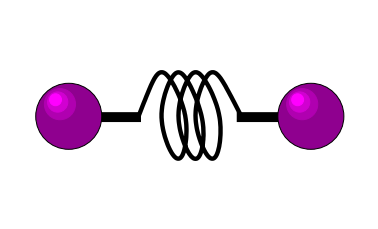
\includegraphics[width=\textwidth]{Figures/Chapter2/bond.png}
    \caption{Bond stretching force-field representation}
    \label{fig:bond}
    \end{subfigure}
    \hspace{1cm}
    \begin{subfigure}[t]{0.25\textwidth}
    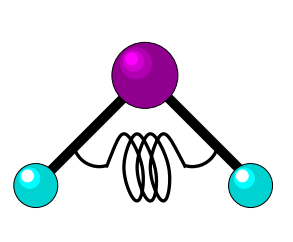
\includegraphics[width=\textwidth]{Figures/Chapter2/angle.png}
    \caption{Bond-angle bending force-field representation}
    \label{fig:angle}
    \end{subfigure}
    
    \begin{subfigure}[t]{0.25\textwidth}
    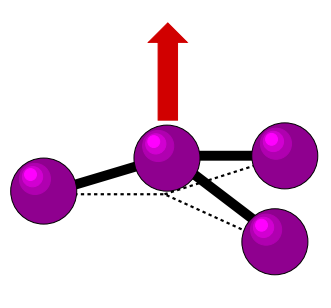
\includegraphics[width=\textwidth]{Figures/Chapter2/impropial.png}
    \caption{Improper dihedral-angle bending force-field representation}
    \label{fig:impropial}
    \end{subfigure}
    \hspace{1cm}
    \begin{subfigure}[t]{0.25\textwidth}
    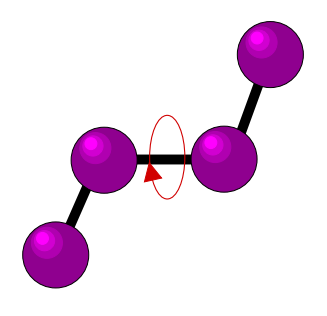
\includegraphics[width=\textwidth]{Figures/Chapter2/torsional.png}
    \caption{Proper dihedral-angle torsion force-field representation }
    \label{fig:torsional}
    \end{subfigure}
    
    
    \caption{Illustration of the various terms included in an empirical potential energy function. Figure adapted from C. Chipot \cite{chipot2010numerical}}
    \label{fig:bonded_inter}
    
\end{figure}

As it is presented in Section \ref{subsec:molecular_structure}, the main objective of this work is to evaluate the non-bonded interactions between the solvent and the solute, particularly the van der Waals interaction. To formulate a complete description of the non-bonded interaction described in Equation \ref{eq:v_general}, the following section is focus on describe the detail mathematical formulation of the terms involved in Equation \ref{eq:nonb_inter}.  

\subsubsection{Force-Field Non-bonded Interactions}

In addition to the bonded interactions between atoms described above, force fields also contain non-bonded interactions. Non-bonded interactions act between atoms in the same molecule and those in other molecules. Force fields usually divide non-bonded interactions into two: Electrostatic interactions and van der Waals interactions.

\subsubsection*{Electrostatic Interactions}
Electrostatic or Coulomb potential describes the interactions potential between pairs of partial charges and it's given by de Coluomb's law.
\begin{equation}
    V^{elec}(q)=\frac{1}{4\pi\epsilon_{0}\epsilon_{1}}\sum_{i=1}^{N-1}\sum_{j=i+1}^{N}\frac{q_{i}q_{j}}{r_{ij}}
    \label{eq:electrostatic}
\end{equation}
where $\epsilon_{0}$ is the dielectric permittivity of vacuum, $\epsilon_{1}$ the relative permittivity of the medium, $q_{i}$ and $q_{j}$ are the charges of atoms $i$ and $j$ involved in the interaction, and $r_{ij}$ the distance between the atoms. 

\subsubsection*{Van der Waals Interactions. The Lenard-Jones Potential}\label{subsubsec:LJ}
The van der Waals force is a weak, short-range force that arises from temporal fluctuations of the charge distribution. This force can attract ideal gas atoms together. Ideal gas atoms are electrically neutral (Figure \ref{fig:vdw_1}) so there is no Coulomb attraction between them. The average dipole moment of an ideal gas atom is zero but the charge fluctuates around its average position and can temporarily create a dipole moment (Figure \ref{fig:vdw_2}). This dipole moment induces a response in the neighboring atom such that there is a net attractive force between the atoms (Figure \ref{fig:vdw_3}). The average over the attractive forces caused by the charge fluctuations is the van der Walls force.

\begin{figure}
    \centering
    \begin{subfigure}[t]{0.25\textwidth}
    
\includegraphics[width=\textwidth]{Figures/Chapter2/vdw1.png}
    \caption{Graphic representation of two neutral atoms.}
    \label{fig:vdw_1}
    \end{subfigure}
    \hspace{0.5cm}
    \begin{subfigure}[t]{0.25\textwidth}
    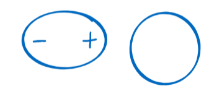
\includegraphics[width=\textwidth]{Figures/Chapter2/vdw2.png}
    \caption{A charge fluctuation creates a dipole.}
    \label{fig:vdw_2}
    \end{subfigure}
    \hspace{0.5cm}
    \begin{subfigure}[t]{0.25\textwidth}
    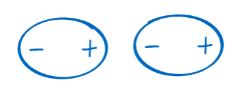
\includegraphics[width=\textwidth]{Figures/Chapter2/vdw3.png}
    \caption{The dipole induces a dipole on the other atom.}
    \label{fig:vdw_3}
    \end{subfigure}
   
    \caption{Illustration of the sequence of events that generates the Van der Waals forces.}
    \label{fig:van_der_waals}
\end{figure}

The Van der Waal bond potential is often approximated by a Lennard-Jones model which consist of two components: a steep repulsive term, $(\sigma/r_{ij})^{12}$ and a smoother attractive term, $(\sigma/r_{ij})^{6}$ as it is shown in Figure \ref{eq:LJ_pot}, which respectively denote repulsive and attractive force. The mathematical description of this potential is given by: 
\begin{equation}
    V^{vdw}(r_{ij})=4\epsilon\left [\left ( \frac{\sigma}{r_{ij}} \right )^{12}-\left (\frac{\sigma}{r_{ij}} \right )^{6} \right ] 
    \label{eq:LJ_pot} 
\end{equation}
where $\epsilon$ is the well depth and a measure of how strongly the two particles attract each other, and $\sigma$ is the distance at which the inter-molecular potential between the two particles is zero as it's shown in Figure \ref{fig:LJ_1}. It gives a measurement of how close two non-bonding particles can get and $r_{ij}$ is the distance of separation between both particles measured from the center of one particle to the center of the other particle.
\begin{figure}[h]
    \centering
    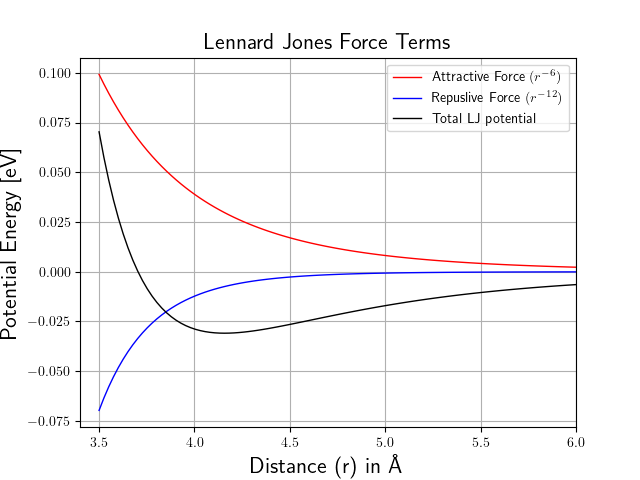
\includegraphics[scale=0.6]{Figures/Chapter2/LJ_1.png}
    \caption{Graphic representation of the attractive and repulsive terms of the Lenard Jones Potential}
    \label{fig:LJ_1}
\end{figure}

Like the bonding potential energy, the stability of an arrangement of atoms is a function of the Lennard-Jones separation distance. As the separation distance decreases below equilibrium, the potential energy becomes increasingly positive (indicating a repulsive force). Such a large potential energy is energetically unfavorable, as it indicates an overlapping of atomic orbitals. However, at long separation distances, the potential energy is negative and approaches zero as the separation distance increases to infinity (indicating an attractive force). This indicates that at long-range distances, the pair of atoms or molecules experiences a small stabilizing force. Lastly, as the separation between the two particles reaches a distance slightly greater than $\sigma$, the potential energy reaches a minimum value (indicating zero force) which is represented by $r_{min}$ in Figure \ref{fig:LJ_parameters}. At this point, the pair of particles is most stable and will remain in that orientation until an external force is exerted upon it. 
\begin{figure}[h]
    \centering
    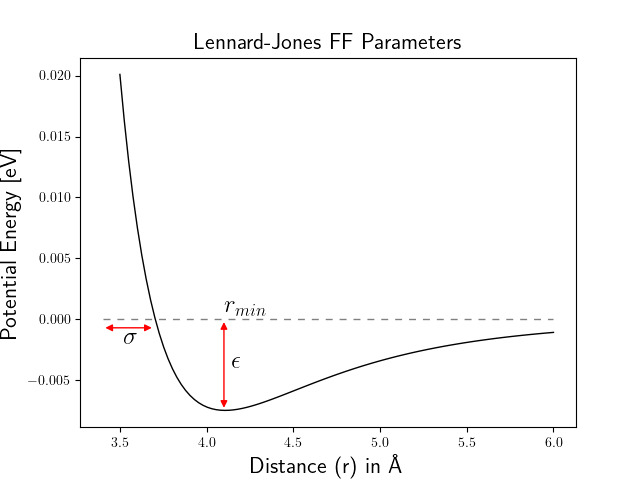
\includegraphics[scale=0.6]{Figures/Chapter2/LJ_2.png}
    \caption{The Lennard-Jones Potential curve, calculated for $\epsilon$ = 0.0103 and $\sigma$ = 3.8.}
    \label{fig:LJ_parameters}
\end{figure}
\begin{equation}
    r_{min}(ij)= 2^{1/6}\sigma
    \label{eq:r_min}
\end{equation}

There are several different ways to formulate the Lennard-Jones potential besides Equation \ref{eq:LJ_pot}, the most common form in the literature is the \textbf{AB potential} and is frequently used in implementations of simulation software as it is computationally favorable. The Lennard-Jones potential can be written as:
\begin{equation}
    V^{LJ}(r_{ij})=\frac{A}{r_{ij}^{12}}-\frac{B}{r_{ij}^{6}} 
    \label{eq:AB_LJ_pot}
\end{equation}
where 
\begin{align*}
    A&=4\epsilon\sigma^{12} & B&=4\epsilon\sigma^{6} & \sigma&=\sqrt[6]{\frac{A}{B}} & \epsilon&=\frac{B^{2}}{4A}
\end{align*}
In GROMOS, the van der Waals (vdw) interaction term $V^{vdw}$ in Equation \ref{eq:nonb_inter} is represented by a Lennard-Jones function, and the term is partitioned as a sum of two contributions. It's given by:
\begin{equation}
    V^{vdw}(r_{ij})=\sum_{i=1}^{N-1}\sum_{j=i+1}^{N} \left [  \frac{C_{12}(i,j)}{r_{ij}^6}-C_{6}(i,j) \right ]\cdot \frac{1}{r_{ij}^6}
    \label{eq:gromos_LJ}
\end{equation}
and every $C_{12}(i,j)$, $C_{6}(i,j)$ is easily extracted from the force-field parameters file in the GROMOS software. More about how GROMOS work is discussed in Section \ref{subsec:about_}. Finally, the total potential energy involved in the therm $V(q)$ from Equation \ref{eq:hamiltonian} it's determined by the sum of every potential energy described in this section, for the pair of atoms $(i,j)$.



\subsection{Configurations of Atoms}
The search of configuration space can be expanded by applying the molecular dynamics (MD) computer simulation technique. Applying MD the classical Newtonian equations of motion of all atoms in the system are solved. These are for a set of N atoms with masses $N_i$ and Cartesian position vectors $r_i (i=1,2,...,N)$. The expression is given by:
\begin{equation}
    \frac{d^{2}r_i(t)}{dt^2}=m_{i}^{-1} F_i(r_1(t),r_2(t),...,r_N(t))
    \label{eq:Newton}
\end{equation}
where the force applied to each atom of the system is obtain by:

These equations can be numerically integrated using small (\~$10^{15}s$) time-steps $\Delta t$ producing a trajectory (atomic positions as a function of time t) of the system \cite{van1988role}.

Regarding the method to generate configurations, the formulation of the energy of the system (Equation \ref{eq:hamiltonian}) which is determined by the molecular system by the force-field, gives the mathematical description of the potential energy described in Equation \ref{eq:Potential}. 
\begin{equation}
    \frac{\partial H}{\partial p_i}=\frac{dq_i}{dt}
    \label{eq:dHdp}
\end{equation}
\begin{equation}
    \frac{\partial H}{\partial q_i}=-\frac{dp_i}{dt}
    \label{dHdq}
\end{equation}
These two derivation from the Hamiltonian gives the velocity (Equation \ref{eq:dHdp}) and as the kinetic energy of the system is not explicitly dependent on positions, Equation \ref{dHdq} is an alternative way to express Equation \ref{eq:Potential}.

These equations describe the physical basis for molecular dynamics (MD) simulations, which integrate these equations as a function of time, for each degree of freedom (for N particles there are 3 position and 3 momentum coordinates, for a total of 6N degrees of freedom). A common alternative is the Monte Carlo (MC) method which is based on random non physical moves to sample an energy distribution. However, MC simulations can be problematic when an explicit solvent is used, as when solvent molecules are simulated along with the molecules of interest problems arise as the solvent restricts movement within traditional MC methods leading to poor sampling when compared to MD methods \cite{wang2008calculation}.

%MD algorithms 
\subsection{Boundary Conditions}
The last aspect to consider in a MD simulation is the boundary conditions, understanding this as how the physical limits of the system or the spatial boundaries and external forces are modeled, and the properties of where , in reality, biologically interesting molecules are found in solvents and cells. When it comes to selecting boundary conditions, there are many options to consider with their own advantages, disadvantages, and computational cost (see Figure \ref{fig:boundary_conditions}). 
\begin{figure}[h]
    \centering
    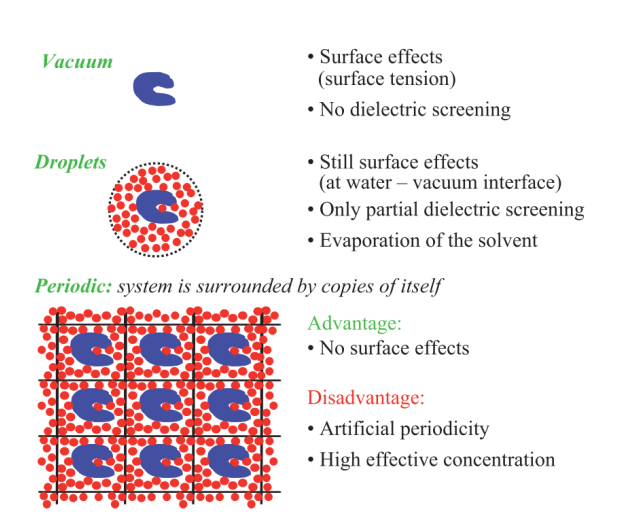
\includegraphics[scale=0.5]{Figures/Chapter2/Boundary_conditions.png}
    \caption{Three types of spatial boundary conditions used in molecular
simulation. Figure from Van Gunsten et al \cite{van2006biomolecular}}
    \label{fig:boundary_conditions}
\end{figure}
The simplest form of boundary conditions is to just simulate the molecule(s) of interest in a vacuum, however this is not representative of molecules in biological conditions and causes many problems in the surface of the molecule.
The next level of detail, and the boundary condition selected for this work because of the property that is evaluated, is when a molecule can be solvated in a droplet of solvent whit a specific geometry. However, this transfers complications from the solute-vacuum interactions to solvent-vacuum interactions, and a ``wall" must be created by fixing the position of the external solvent molecules, so that they don’t evaporate.
The method usually considered most appropriate for biological simulations is periodic boundary conditions, where the system is surrounded in all directions by copies of itself, removing surface effects and emulating bulk conditions. 
\subsection{General Molecular Dynamics Algorithm}

Starting with a given number of atoms $``N"$, one want to be able to simulate or predict how those atoms will be moving according to time. What will be the displacement or trajectory of these atoms at a different time. The algorithm works as follows:
\begin{enumerate}
    \item System Initial Configuration $\vec{r_{i}}(t=0)$ ; $\vec{v_{i}}(t=0)$\\
    Given a system of $``N"$ atoms, initial position vectors $\vec{r_i}$ and initial velocity vectors $\vec{v_i}$ at $t=0$, with $i=\{1,2,3,...,N\}$, are generated depending on the system configuration. In Section  \ref{subsec:about_} is explained how GROMOS software generates data sets for both initial position and initial velocities by minimisation and termalization processes respectively.
    \item Total Potential Energy $U_{ij}$ \\
    Given the initial configuration of the system, the inter-atomic potential energy between atoms now can be determined. Each pair of atoms potentially will have a given energy between them $U_{ij}$ because of the forces applied $\vec{F_{ij}}$. This interaction is determined by electrostatic (Equation \ref{eq:electrostatic}) and Van der Waals (Equation \ref{eq:LJ_pot}) forces and is intrinsically dependent on the distance between them $r_{ij}$. The total potential energy is equal to the sum of each pair interaction between atom $i$ and $j$.
    $$U_{tot}=\sum_{i\neq j}^N U_{ij}$$
    \item Determine Total Forces Applied\\
    With the potential energy $U_{ij}$ as a function of the distance $r_{ij}$ between two atoms, the force apply by a given atom $i$ on atom $j$ can be calculated by the gradient of the energy.
    $$ F_{i\rightarrow j}=-\vec{\triangledown } U_{ij}$$
    $$ \vec{F_i} = \sum_{i\neq j}^N F_{i\rightarrow j}$$
    Therefore, the resultant force on an atom $i$ must be the sum of all forces between it and all other atoms $j\neq i$. 
    \item Acceleration on each atom.\\
    Applying Newton's equations of motion and knowing the forces and the masses of each individual atom,  the acceleration applied on each atom is given by:
    $$\vec{a_i}=\frac{\vec{F_i}}{m_i}$$
    \item Prediction of Motion $r(t+dt)$ ; $v(t+dt)$\\
    Knowing the initial position and initial velocity of an atom $i$, and knowing it's acceleration one can predict how the atoms will be moving after a small increment of time $dt$. Now, one can calculate the new velocity $v(t+dt)$ and new position $r(t+dt)$ after a small increment in time. This relies on the numerical integration. Knowing the acceleration, it can be integrating in order to get the position and how the position is changing according to time. 
\end{enumerate}
Figure \ref{fig:md_algo} summarizes the algorithm described above. 
\begin{figure}[h]
    \centering
    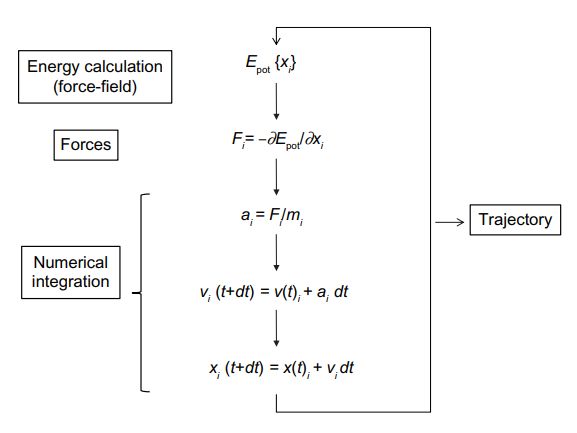
\includegraphics[scale=0.5]{Figures/Chapter2/md_algorithm.png}
    \caption{Molecular dynamics basic algorithm. Figure from Hospital \textit{et al.} \cite{hospital2015molecular}}
    \label{fig:md_algo}
\end{figure}

\subsubsection{Numerical Integration}\label{subsubsec:leapfrog}
Multiple methods to integrate equations of motion have been developed. Among these is the \textbf{leap-frog algorithm} \cite{leach2001molecular} which was used for the simulations carried out in this work. Figure \ref{fig:leapfrog} is a schematic representation of how the variables for velocities and positions are compute throw the mathematical scheme \cite{cuendet2007calculation}. 
\begin{figure}
    \centering
    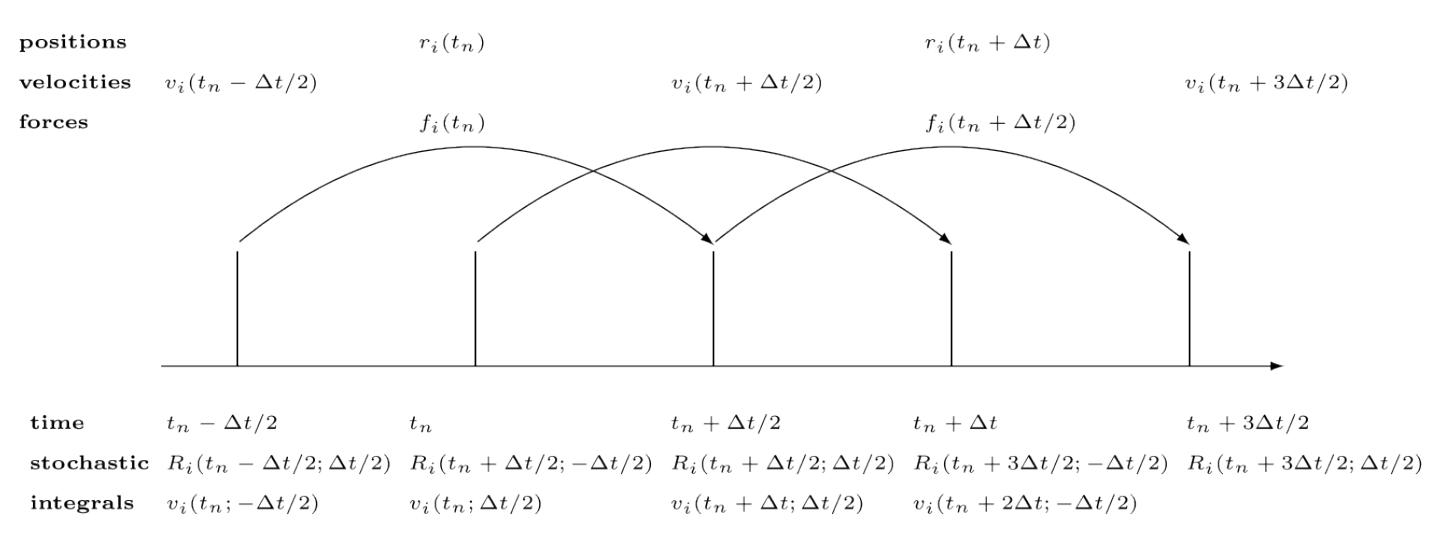
\includegraphics[scale=0.31]{Figures/Chapter2/Leap_Frog.png}
    \caption{The leap-frog integration scheme.Figure from Van Gunsteren: Gromos Manual Vol.2}
    \label{fig:leapfrog}
\end{figure}
When a Taylor expansion of the velocity $v_i(t_n-\Delta t/2)$ at $t=t_n$ is subtracted from
an expansion of $v_i(t_n+\Delta t/2)$ at $t=t_n$, neglecting terms of third and higher order for simplicity, results: 
\begin{equation}
    v_i(t_n+\Delta t/2) = v_i(t_n-\Delta t/2) + \frac{F_i(t_n)}{m_i}\Delta t
    \label{eq:v_i_tylor}
    \end{equation}
And similarly, when a Taylor expansion of the position $r_i(t_n)$ at $t=t_n + \Delta t/2$ is subtracted from an expansion of $r_i(t_n + \Delta t)$ at $t=t_n + \Delta t/2$ results (again neglecting terms of third and higher order for simplicity):
\begin{equation}
    r_i(t_n + \Delta t)=r_i(t_n) + v_i(t_n = \Delta t/2) \Delta t
    \label{eq:r_i_tylor}
\end{equation}
Equations \ref{eq:v_i_tylor} and \ref{eq:r_i_tylor} are the leap-frog velocity and position formulas, respectively, which together form the leap-frog scheme. This provides a simple method where a MD algorithm alternates between calculating (and updating) positions and velocities.


\section{Implicit Solvent Models}\label{sec:implicit}
\vspace{3cm}
\par
As it is mentioned in Section \ref{sec:MD}, interactions between a solute molecule and a surrounding solvent are of fundamental importance across chemistry, biology, and associated fields of science and engineering. Fully atomistic, explicit-solvent MD simulations provide an accurate and chemically detailed understanding of these interactions therefore they can be can be highly demanding in the consumption of computational resources. This cost is is associated with the large number of solvent molecules required to model a bulk solution. In practical situations, a large fraction of the time is spent calculating a detailed trajectory of the solvent molecules, even though it is primarily the solute behavior that is of interest.

Because of this, it is desirable to develop different approaches in which the influence of the solvent is incorporated \textbf{implicitly}. Approximate schemes treating the solvent implicitly can provide useful quantitative estimates and remain computationally inexpensive \cite{roux1999implicit} \cite{zacharias2003continuum}.

\subsection{Implicit model: Solvation Free Energy}

Solvation is the process of reorganizing solvent and solute molecules into solvation systems. Solvation involves bond formation, hydrogen bonding, and van der Waals forces. Solvation of a solute by water is called hydration \cite{campbell2006chemistry}. The solvation process describes the interaction between the solute and solvent molecules. This process will be thermodynamically favored only if the overall Gibbs energy of the solution is decreased, compared to the Gibbs energy of the separated solvent and solid (or gas or liquid). Regarding Equation \ref{eq:Gibbs}, a negative Gibbs energy indicates a spontaneous process but does not provide information about the rate of dissolution.

This process involves multiple steps with different energy consequences: First, a cavity must form in the solvent to make space for a solute (Figure \ref{fig:solv_1} to Figure \ref{fig:solv_2}). This is both entropically and enthalpically unfavorable, as solvent ordering increases and solvent-solvent interactions decrease. Stronger interactions among solvent molecules leads to a greater enthalpic penalty for cavity formation. Next, a particle of solute must separate from the bulk. This is enthalpically unfavorable since solute-solute interactions decrease, but when the solute particle enters the cavity, the resulting solvent-solute interactions are enthalpically favorable. 

\begin{figure}[h]
    \centering
    \begin{subfigure}[t]{0.25\textwidth}
    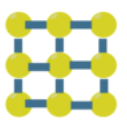
\includegraphics[width=\textwidth]{Figures/Chapter 4/Cavity_1.png}
    \caption{Representation of bulk solvent.}
    \label{fig:solv_1}
    \end{subfigure}
    \hspace{0.5cm}
    \begin{subfigure}[t]{0.25\textwidth}
    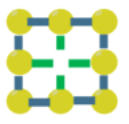
\includegraphics[width=\textwidth]{Figures/Chapter 4/Cavity_2.png}
    \caption{A cavity with the solute geometry is form in the solvent.}
    \label{fig:solv_2}
    \end{subfigure}
    \hspace{0.5cm}
    \begin{subfigure}[t]{0.25\textwidth}
    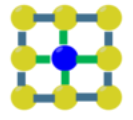
\includegraphics[width=\textwidth]{Figures/Chapter 4/Cavity_3.png}
    \caption{The solute is placed in the solvent cavity with the respective solute-solvent interactions}
    \label{fig:solv_3}
    \end{subfigure}
   
    \caption{Representation of the solvation process for any molecule in solution.}
    \label{fig:solvation}
\end{figure}
The solvation free energy, process described in Figure \ref{fig:solvation}, is frequently decomposed as a sum of \textit{polar} $(\Delta G_{polar})$ and \textit{non-polar} $(\Delta G_{np})$ terms  \cite{zacharias2003continuum}. 
\begin{equation}
    \Delta G^{solv} = \Delta G_{polar}^{solv} + \Delta G_{np}^{solv}
    \label{eq:G_solv}
\end{equation}
The polar term is the free energy of creating the solute’s charge distribution inside a pre-existing solute cavity, Assuming a charge distribution given by a molecular mechanics force field, the polar solvation contribution can be modeled with macroscopic continuum dielectric theory, e.g. the Poisson-Boltzmann equation. This works focuses on the \textbf{non-polar} component which is define as the work required to place an uncharged solute inside the solvent and generates a dry cavity on it. This contribution is often estimated from the solvent accessible surface area (SASA) of the molecule using a uniform surface tension coefficient obtained from a fit of experimental \cite{zacharias2003continuum}. 

\subsubsection{Solvent-Accessible Surface Area (SASA) Model}\label{subsubsec:SASA_model}
Implicit-solvent models often treat $\Delta G_{np}$ as a weighted combination of the solute’s SASA and other geometric measures given by: 
\begin{equation}
    \Delta G_{np} = \gamma (SASA) + b
    \label{eq:SASA}
\end{equation}
where $\gamma$ is is usually interpreted as the liquid-vapor surface tension, and $b$ is a scaling constant. Geometrically, \textit{Solvent Accessible Surface Area} is related to the region of the molecule surface exposed enough to be able to interact with solvent molecules. It is usually defined as a surface built by the delineation drawn by the center of a sphere (rough representation of a solvent molecule, usually of 1.4 [\r{A}] radii; i.e. a water molecule) rolling over the molecular surface. 
Nevertheless, the accurate prediction of the solvation free energy remains a very challenging issue and several inaccuracies with this method have been presented by some authors \cite{gallicchio2000enthalpy} \cite{wang2018breaking},  suggesting that an empirical parametrization of the hydration free energy and the free energy of association of apolar species based only on the solvent accessible surface area is insufficient. Successful parametrization should contain a surface area term to reproduce effects due to entropy loss and solvent reorganization energy and terms that depend on the number, location, and type of atomic interaction centers to reproduce effects due to the solute-solvent dispersion interactions which are only weakly correlated with surface area. 










\subsection{Non-polar Solvation Free Energy Estimation}\label{subsec:CC_method}

The non-polar term in Equation \ref{eq:G_solv} can itself be decomposed into a sum of two free energies \cite{zacharias2003continuum}, $\Delta G_{cav}$ the creation of a solute-shaped cavity by turning on the potential short-range \textbf{repulsive interactions}, and $\Delta G_{disp}$, in which one turns on the longer-range \textbf{attractive} solute-solvent dispersion interactions.
\begin{equation}
    \Delta G_{np}=\Delta G_{cav} + \Delta G_{disp}
    \label{eq:G_np}
\end{equation}
Traditionally, $\Delta G_{cav}$ is highly correlated with the SASA factor previously described, however, the value of $\gamma$ does not agree with the surface tension coefficient and works as a adjustable parameter which can change the errors. On the other hand, $\Delta G_{disp}$ can be described with a continuum model, where the solute-solvent dispersion interaction potential is integrated over the solvent, which in turn can be formulated as an volume integral over the solvent accessible surface \cite{tan2007implicit}.
It is been study that while repulsive and attractive components of the non-polar part both scale roughly with surface area (or volume) of the solute, the total non-polar free energy does not scale with the solute surface area or volume. \cite{mobley2009small}.

\subsubsection{Implicit Solvent Model for $\Delta G_{cav}$ and $\Delta G_{disp}$}
A new approach to estimate $\Delta G_{cav}$ and $\Delta G_{disp}$ \cite{} proposes an implicit solvent model with a clearer physical meaning than current available models. Regarding Equations \ref{eq:G_solv} and \ref{eq:G_np}, the non-polar solvation free energy can be expressed as (See Figure \ref{fig:np_cycle}): 
\begin{equation}
    \Delta G_{solv}= \Delta G_{cav}+ \Delta G_{disp}+ \Delta G_{polar}
\end{equation}
\begin{figure}[h]
    \centering
    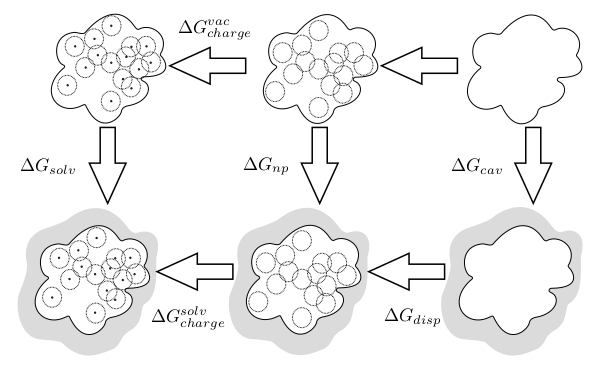
\includegraphics[scale=0.6]{Figures/Chapter 4/np_cycle.png}
    \caption{Thermodynamic cycle for solvation energy. Figure taken from \cite{cooper2020simple}}
    \label{fig:np_cycle}
\end{figure}

Using a capacitance-based approach for $\Delta G_{cav}$, the potential inside the solute is model as a constant $\phi_{static}$, defining the solute boundary as the solvent-excluded surface (SES) \cite{connolly1983analytical}. In the infinite solvent region, the potential is model as $\phi=0$, and bound the region using the boundary of the first solvation shell (the solvent-accessible surface, SAS \cite{connolly1983analytical}. These surfaces bound a shell, which is model as a macroscopic dielectric with the uniform relative permittivity $\epsilon_{shell}$, and where the electrostatic potential obeys the Laplace equation. Fixing the potentials at both boundaries implies that the dielectric constants of the solute and bulk solvent are irrelevant.. It is used $\epsilon_{shell}$ as a fitting parameter, but it has clear physical bounds and significance. The energy associated with this boundary-value problem can be solved using a pair of coupled boundary-integral equations for unknown charge densities on the two surfaces by: 
\begin{equation}
    \begin{bmatrix}
V_{diel} & V_{diel}\\ 
 V_{shell}& V_{shell}
\end{bmatrix}\begin{bmatrix}
\sigma_{diel}\\ 
\sigma_{shell}
\end{bmatrix}
=
\begin{bmatrix}
\phi_{static}\\ 
0
\end{bmatrix}
\end{equation}
where $V_{diel}(\phi_{shell})=\oint_{shell}\frac{\phi(r')}{4\pi\left |r_{diel}-r' \right |}$ denotes the potential induced at the inner surface (the dielectric boundary) by the surface charge distribution on the outer boundary (the solvent-accessible surface). Figure \ref{fig:capacitor} represent this idea. 
\begin{figure}[h]
    \centering
    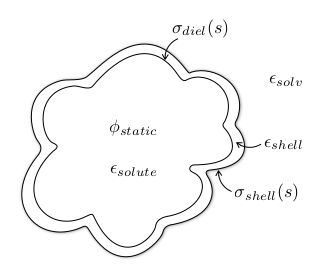
\includegraphics[scale=0.5]{Figures/Chapter 4/capacitor_model.png}
    \caption{Sketch of the capacitor model. Figure taken from \cite{cooper2020simple}}
    \label{fig:capacitor}
\end{figure}
Having found the surface charge distributions it is possible to compute the work (and hence, the free energy) required to charge the resulting capacitor with standard electrostatic theory
\begin{equation}
    \Delta G_{cav}=\int_{\Omega}\phi(r)\rho(r)dr
    \label{eq:g_cav}
\end{equation}
being $\rho$ the charge distribution, in this case, concentrated on the SAS ($\sigma_{shell}$) and SES ($\sigma_{diel}$)Noting that the potential on the outer surface is zero, we can rewrite Equation \ref{eq:g_cav} as: 
\begin{equation}
    \Delta G_{cav}=\oint_{diel}\phi_{static}\sigma_{diel}(r)dr
    \label{eq:int_shell}
\end{equation}

The previous $\Delta G_{cav}$ component is combine with a modification of a continuum integral method \cite{levy2003nonpolar} for calculating $\Delta G_{disp}$, by integrating the Lennard-Jones potential outside the solvent-accessible surface which can be formulated as a surface integral using the divergence theorem by: 
\begin{equation}
    \Delta G_{disp}=\sum_i \oint_{shell} \rho_w \frac{\partial}{\partial n}\left ( \frac{A_i}{90\left |r-r_i\right |^{10}} - \frac{B_i}{12\left |r-r_i\right |^{4}} \right )dr
    \label{eq:CC_implicit}
\end{equation}
where $\rho_w$ is considered to be the bulk number density, $A_i$ and $B_i$ re related to the Lennard-Jones parameters for the water oxygen and atom i, the sum is over the solute’s atoms, and the unit vector \textbf{n} points into the solvent.
Finally, a solvation-layer interface condition (SLIC) continuum electrostatics method   \cite{mehdizadeh2019solvation} is used to compute $\Delta G_{polar}$ (or $\Delta G_{charge}^{solv}$ in Figure \ref{fig:np_cycle}). (Notice that regarding the thermodynamic cycle represented in Figure \ref{fig:np_cycle},  $ \Delta G_{solv}$ is equivalent to $\Delta G_{charge}^{solv}$ - $\Delta G_{charge}^{vac}$).



 
\section{Free Energy}\label{sec:Free_energy}
\vspace{3cm}
\par


The free energy is a highly desirable quantity to compute. It is in essence the factor that determines how a process will proceed and the probability that a system will adopt a given state. The ability to calculate free energies from molecular simulations not only allows one to understand the underlying processes on an atomic level but also to probe states of a system not accessible experimentally. In particular, if precise and accurate estimates of the free energy of a system could be obtained directly from numerical simulations, the need to measure thermodynamic properties of a system, such as ligand-binding constants \cite{free_energy}, by experiment would be greatly reduced. This is why, for example, free energy calculations have attracted much interest in areas such as rational drug design and material science. 
Free energy calculations can be classified into two categories. The calculation of conformational free energies aims at evaluating the relative free energies of relevant conformational states of a given molecular system. The calculation of alchemical free energies on the other hand aims at evaluating the relative free energies of different molecules, which is the main objective of this work. 

Free energy is an extensive property, meaning that its magnitude depends on the amount of a substance in a given thermodynamic state, and it's expressed in two forms depending on the conditions that it is determined: The relative (Helmholtz) free energy $F$ is obtained under isochoric-isothermic conditions (NVT), whereas the relative (Gibbs) free enthalpy $G$ is obtained under isobaric-isothermic conditions (NPT). Both expressions are given by: 
\begin{equation}
    F=U-TS
    \label{eq:Helmholtz}
\end{equation}
\begin{equation}
    \begin{split}
    G&=U+PV-TS\\ 
     G&=H-TS
    \end{split}
    \label{eq:Gibbs}
\end{equation}

From an MD trajectory, described in Section \ref{sec:MD}, the statistical equilibrium averages can be obtained for any desired property of the molecular system for which a value can be computed at each point of the trajectory. Examples of such properties are the potential or kinetic energy of relevant parts of the system, structural properties and fluctuations, electric fields, diffusion constants, etc. A number of thermodynamic properties can be derived from such averages. However, two important thermodynamic quantities, the entropy and the (Gibbs or Helmholtz) free energy, generally cannot be derived from a statistical average. They are global properties that depend on the extent of phase (or configuration) space accessible to the molecular system \cite{van1988role}. Fortunately, with statistical mechanics methods one can evaluate the \textit{relative} free energy differences.


\subsection{Thermodynamic Integration}\label{subsec:TI}

The aim of thermodynamic integration is to compute the difference in a thermodynamic property (usually the free energy) of the system between some reference state and the state of interest. It make use of the fact that the free energy changes related to small perturbations of a molecular system can be determined during a simulation. Taking that fact into account, the free energy difference between two states A and B of a system can be determined from an MD simulation in which the potential energy function $V(q)$ is slowly changed such that the system slowly changes from state A to state B over a reversible path.

Since the absolute value for free energy of solvation is difficult to calculate directly, we use the fact that the free energy is a \textbf{state function}. From the thermodynamic cycle presented in Figure \ref{fig:TI_cicle} it follows that:
\begin{figure}[h]
    \centering
    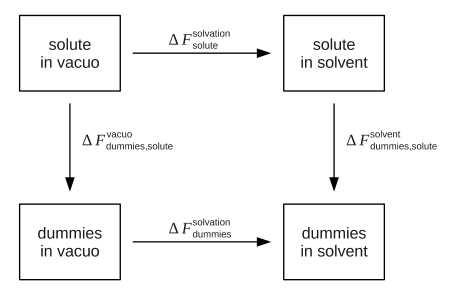
\includegraphics[scale=0.6]{Figures/Chapter 3/Ciclo_termodinamico.png}
    \caption{Thermodynamic cycle for the determination of solvation free energies}
    \label{fig:TI_cicle}
\end{figure}

\begin{equation}
    \Delta F_{solute}^{solvation} = \Delta F_{dummies,solute}^{vacuo} + \Delta F_{dummies}^{solvation} - \Delta F_{dummies,solute}^{solvent} 
\end{equation}  
The solvation free energy $\Delta F_{solute}^{solvation}$ is the work required to transfer a molecule from the gas phase into solute solution. $\Delta F_{dummies,solute}^{vacuo}$ is the work required to remove all the internal nonbonded interactions in the solute in vacuo, which is achieved by gradually mutating all atoms in a solute molecule into dummy atoms. A dummy atom is an atom for which the nonbonded interactions, i.e. Lennard-Jones and electrostatic interactions, with all other atoms are set to zero while the bonded interactions within the molecule and the masses of individual atoms are kept unchanged. $\Delta F_{dummies}^{solvation}$ is the work required to transfer the dummy solute molecule from
vacuum to the solvated phase. As the dummy molecule does not interact with the rest of the system this
term is also equal to zero. In order to determine the solvation free energy of any peptide with this method, only the free energy $\Delta F_{dummies,solute}^{solvent}$ must therefore be calculated. Since $\Delta F_{dummies,solute}^{solvent}$ is the work required to remove the solute-solvent and solute-intermolecular interactions. for this particular case, as we are interesting only in the solute-solvent interaction (Van der Waals) the intermolecular forces between the peptide atoms remain constant. 

This transition, from a particular atom to a dummy particle, works as follows:
\textbf{(1)} The Hamiltonian $H(p,q)$ is made a function of a coupling parameter $\lambda$, such that $H(p,q,\lambda)$ characterises the two different sates of interest, normal and dummy particle. 
\begin{equation}
    H(p,q,\lambda)=\sum^N_{i=1}\frac{p_i^2}{2m_i(\lambda)}+V(q,\lambda)
    \label{eq:Ham_lambda}
\end{equation}
with
\begin{equation}
    m_i(\lambda)=(1-\lambda)m_i^A +\lambda m_i^B
\end{equation}
and
\begin{equation}
    \begin{split}
        V(q,\lambda) &= \sum_{bonds,b} V(b,\lambda) + \sum_{angles,\theta} V(\theta,\lambda) + \sum_{torsion,\xi} V(\xi,\lambda)  + \\
        &   + \sum_{dihedrals,\xi} V(\psi,\lambda) + \sum_{nonb (i,j)} V(r_{ij},\lambda)
    \end{split}
    \label{eq:V_lambda}
\end{equation}

Equation \ref{eq:V_lambda} represents each one of the potential energy terms described in Equations \ref{eq:bond_inter} and \ref{eq:nonb_inter} with the couple parameter $\lambda$.
In this work, only the non bonded interaction will be modify with the coupling parameter and study the transition between the twp states. The mathematical formulation will be presented in following sections. 

\subsubsection{Gibbs Free Energy}

The Gibbs free energy of the system becomes a function of $\lambda$ and is given by: 
\begin{equation}
    G(\lambda)=-kT\ln{\Delta \lambda}
    \label{eq:DG_general}
\end{equation}
where $k$ denotes Boltzmann's cosntant, $T$ is the temperature of the system and $\Delta \lambda$ is the isobaric partition function given by: 
\begin{equation}
    \Delta \lambda= \frac{1}{h^{3N}N!}\int\int\int\exp{[(-H(p,q,\lambda)+PV)/kT]}dVdpdq
    \label{eq:part_func}
\end{equation}
where $P$ and $V$ are the pressure and the volume of the system respectively, $p$ and $q$ are the momentum and Cartesian coordinates of the N atoms. 

The free energy difference $\Delta G_{BA}$ is givne by: 
\begin{equation}
    \Delta G_{BA}= G(\lambda_B) - G(\lambda_A) = -kT\ln{\left ( \frac{\Delta \lambda_B}{\Delta \lambda_A} \right )}
\end{equation}
which can be expressed as an ensemble average by:
\begin{equation}
    \begin{split}
       &\Delta G_{BA} =-kT\ln\\\\
       &{\left \{ \frac{\int\int\int\exp{[(-H(p,q,\lambda_B)-H(p,q,\lambda_A))/kT]}\exp{[(-H(p,q,\lambda_A)+PV)/kT]}dVdpdq} {\int\int\int\exp{[(-H(p,q,\lambda_A)+PV)/kT]}dVdpdq} \right \}}\\\\
       &=-kT\ln{\left \{  \left \langle \exp{[(-H(p,q,\lambda_B)-H(p,q,\lambda_A))/kT]} \right \rangle \right \}}
    \end{split}
\label{eq:pertur}
\end{equation}
where the $\left \langle ... \right \rangle_\lambda$ mean an ensemble average over the volume $V$, the coordinates $q$ and momentum $p$ at the value $\lambda$. Equation \ref{eq:pertur} is called the perturbation formula, since only yield accurate results when state B is close to state A. If this difference is large, that change from A to B must be split up into a number of steps between intermediate states that are close enough to allow the use of Equation \ref{eq:pertur} \cite{van1988role}. Meeting this condition, $\Delta G_{BA}$ is just the sum of the individual $\Delta G$ for all intermediate steps. The differentiation of Equation \ref{eq:DG_general} with respecto to $\lambda$ at constant temperature and pressure yields:
\begin{equation}
    \begin{split}
        &\left ( \frac{\partial G(\lambda)}{\partial \lambda} \right )_{T,P}=-\left ( \frac{kT}{\Delta (\lambda)} \right ) \left [ \frac{\partial \Delta (\lambda)}{\partial \lambda} \right ]_{T,P} \\\\
        &=\frac{\int\int\int[\partial H(p,q,\lambda)/\partial \lambda] \exp{[-(Hp,q,\lambda)+PV)/kT] dV dp dq}}{\int\int\int\exp{[-(H(p,q,\lambda)+PV)/kT]dV dp dq}}\\\\
        &=\left \langle \frac{\partial H(p,q,\lambda)}{\partial \lambda} \right \rangle_\lambda
    \end{split}
\end{equation}
The free-energy difference ($\Delta G$) between two states, A and B, can be readily calculated using the TI formula:
\begin{equation}
    \Delta G_{BA}=G(\lambda_{B})-G(\lambda_{A})=\int_{\lambda =0}^{\lambda =1}\left \langle \frac{\partial H(\lambda )}{\partial \lambda } \right \rangle_\lambda d\lambda
    \label{eq:TI}
\end{equation}
 where $H(\lambda)$ is a combined potential energy function connecting the potential energy functions with a coupling parameter $\lambda$ between states $A (H_{A}; \lambda =0) $ and state $B (H_{B}; \lambda =1)$. In this methodology, state A is represent the peptide with the normal peptide-solvent interactions, while state B refers to a non-interacting dummy particle described in the previous paragraph. In the practice, the result of Equation \ref{eq:TI} is computed a every $\lambda$ point and then numerically integrated to obtain the free energy difference between the two states. Figure \ref{fig:GA_to_GB} represent this idea. 
 \begin{figure}[h]
     \centering
     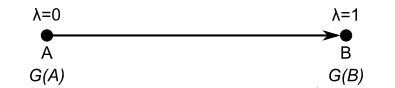
\includegraphics[scale=0.5]{Figures/Chapter 3/GA_to_GB.png}
     \caption{Transition between the states A and B with according to coupling parameter $\lambda$}
     \label{fig:GA_to_GB}
 \end{figure}
 
If $\lambda$ is being changed very slowly from $\lambda_A$ to $\lambda_B$ during a MD simulation, the integration of Equation \ref{eq:TI} can be carried out in the course of the MD run. In this way $\Delta G_{BA}$ can be obtained for rather different states A and B, as long as the continuous change in $\lambda$ is so slow that the system remains essentially in equilibrium for each intermediate value of $\lambda$.

\subsubsection{Soft-Core Potential Energy}\label{subsubsec:softcore}

A practical problem affect the predicted free energy difference and that is the presence of a \textit{"singularity"} in the function for which an ensemble average is to be determined, in this case, the Hamiltonian. When the ensemble average is obtained by MD simulation such singularities may also lead to numerical instabilities in the integration of the equations of motion \cite{beutler1994avoiding}. In general, a singularity problem arises in simulations when an observable, for which the ensemble average is to be calculated, contains regions high-energy regions of the Hamiltonian. Depending on the pathway chosen, the ensemble average of this observable may diverge. The van der Waals interaction and the electrostatic interaction between charges of equal sign (repulsive forces) become infinitely large for $r_{ij}$ approaching zero.  

In the practice, the singularity problem is often encountered when non-bonded interactions sites are to be removed, added or modify. A soft-core potential energy function is employed by GROMOS software to avoid singularities near the end-states of the TI simulations. The Lennard-Jones potential (LJ) energy function, Equation \ref{eq:gromos_LJ}, between atoms $i$ and $j$ at a state $X$ is then defined as:
\begin{equation}
    H^{VdW}_{i,j,\lambda} = \left [ \frac{C_{12}^{X}(i,j)}{\alpha_{LJ}\lambda^{2}C_{12,6}^{X}(i,j)+(r_{ji})^{6}} - C_{6}(i,j)\right ]\cdot \frac{1}{\alpha_{LJ}\lambda^{2}C_{12,6}^{X}(i,j)+(r_{ji})^{6}}
\end{equation}

The singularity at $r_{ij}=0$ is removed and the interaction function is smoothened for $\lambda=0$ and $\alpha_{LJ}$ is the softness parameter for the LJ interaction. A similar transformation is used to couple the $\lambda$ parameter to electrostatic potential (Equation \ref{eq:electrostatic}) and it's given by: 
\begin{equation}
    H^{elec}_{i,j,\lambda}=\frac{q^X_i q^X_j}{4\pi \epsilon_0 \epsilon_1}\left [ \frac{1}{\left [ \alpha_{CRF}(i,j)\lambda^2+r_{ij}^2\right ]^{\frac{1}{2}}} - \frac{\frac{1}{2}C_{rf}r{ij}^2}{\left [\alpha_{CRF}(i,j)\lambda^2+R_{rf}^2 \right ]^\frac{3}{2}} - \frac{\left ( 1-\frac{1}{2}C_{rf}\right )}{R_{rf}}\right ]
    \label{eq:softcorepot}
\end{equation}
where $q_i^X$ is the partial charge of atom $i$ and $C_{rf}$ and $R_{rf}$ are parameters of the reaction-field method \cite{tironi1995generalized}. $\alpha_{CRF}$ is the softness parameter for the electrostatic interactions, similar to $\alpha_{LJ}$ described before. Finally, the non-bonded potential energy for particles $i$, $j$ in a given state (from A to B)is calculated as:
\begin{equation}
    H_{i,j,\lambda}^{NB}= H^{VdW}_{i,j,\lambda}+H^{elec}_{i,j,\lambda}
\end{equation}
The combined non-bonded potential energy function connecting states A and B is now:
\begin{equation}
    H(r_{ij};\lambda)=\lambda H^{NB}(r_{ij};B;(1-\lambda))+(1-\lambda)H^{NB}(r_{ij};A;\lambda)
\end{equation}

Because the focus of the present study is on calculating non-polar contributions to the solvation process, the alanine molecules were treated as neutral without any partial charges on the atoms for simplicity and to avoid any electrostatic contributions to solvation. This was accomplished by set to 0 all the atomic charges of every atom in the \textbf{*.top} file. 

\section{Methods}\label{sec:methods}

%...
\vspace{3cm}
\par
\subsection{Structure Preparation}\label{subsec:strucutre_prep}

In order to study the behavior of non-polar interaction in the solvation process, the free energy calculation, and how these two properties are related to the volume (size) of the molecules, a total of 20 structures were prepared to preform MD simulations using VMD-\texttt{molefacture} plugin \cite{humphrey1996vmd}. This tool has been designed to facilitate the construction and parameterisation of small molecules. It additionally provides a simple interface to prepare structures and files. These structures classifies as follows:
\begin{itemize}
    \item \underline{10 helix $n$-Alanines:} These correspond to the ``natural" configurations of the alanines with curvatures present on they structures. (Figure \ref{fig:5ALAhelix})
    \item \underline{10 extended $n$-Alanines:} They conformation where fixed to maintain a straight configuration along an axis. (Figure \ref{fig:5ALAext})
\end{itemize}   
with $n$ ranging from 1 ($ALA_1$)  to 10 ($ALA_{10}$) in both configurations. The peptide terminals where capped with with neutral amino-terminal ($NH_2$) and C-terminal ($COOH$). From this point, every step was preform using GROMOS molecular simulation software \cite{basharat2016structure}. 

\begin{figure}[h]
    \centering
    \begin{subfigure}[t]{0.45\textwidth}
    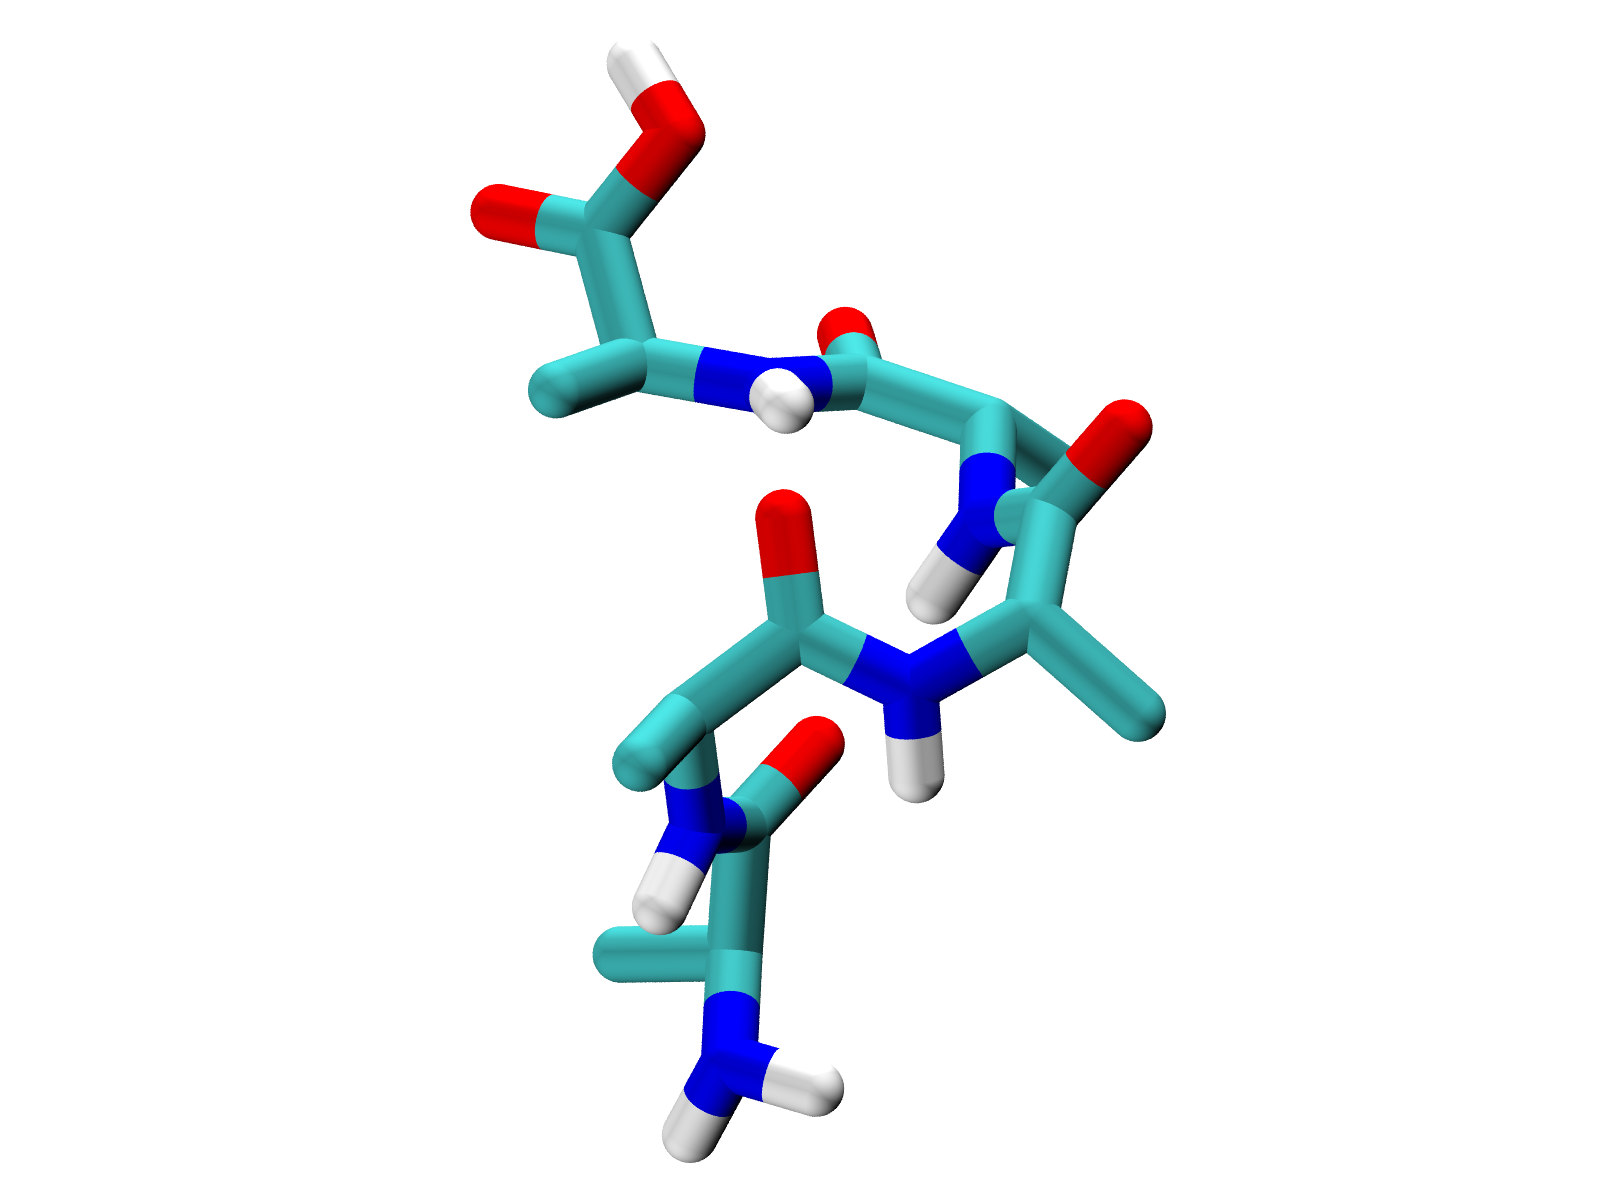
\includegraphics[width=\textwidth]{Figures/Chapter_5/5ALA_helix.png}
    \caption{Representation of helix-($ALA_5$) configuration.}
    \label{fig:5ALAhelix}
    \end{subfigure}
    \hspace{0.5cm}
    \begin{subfigure}[t]{0.45\textwidth}
    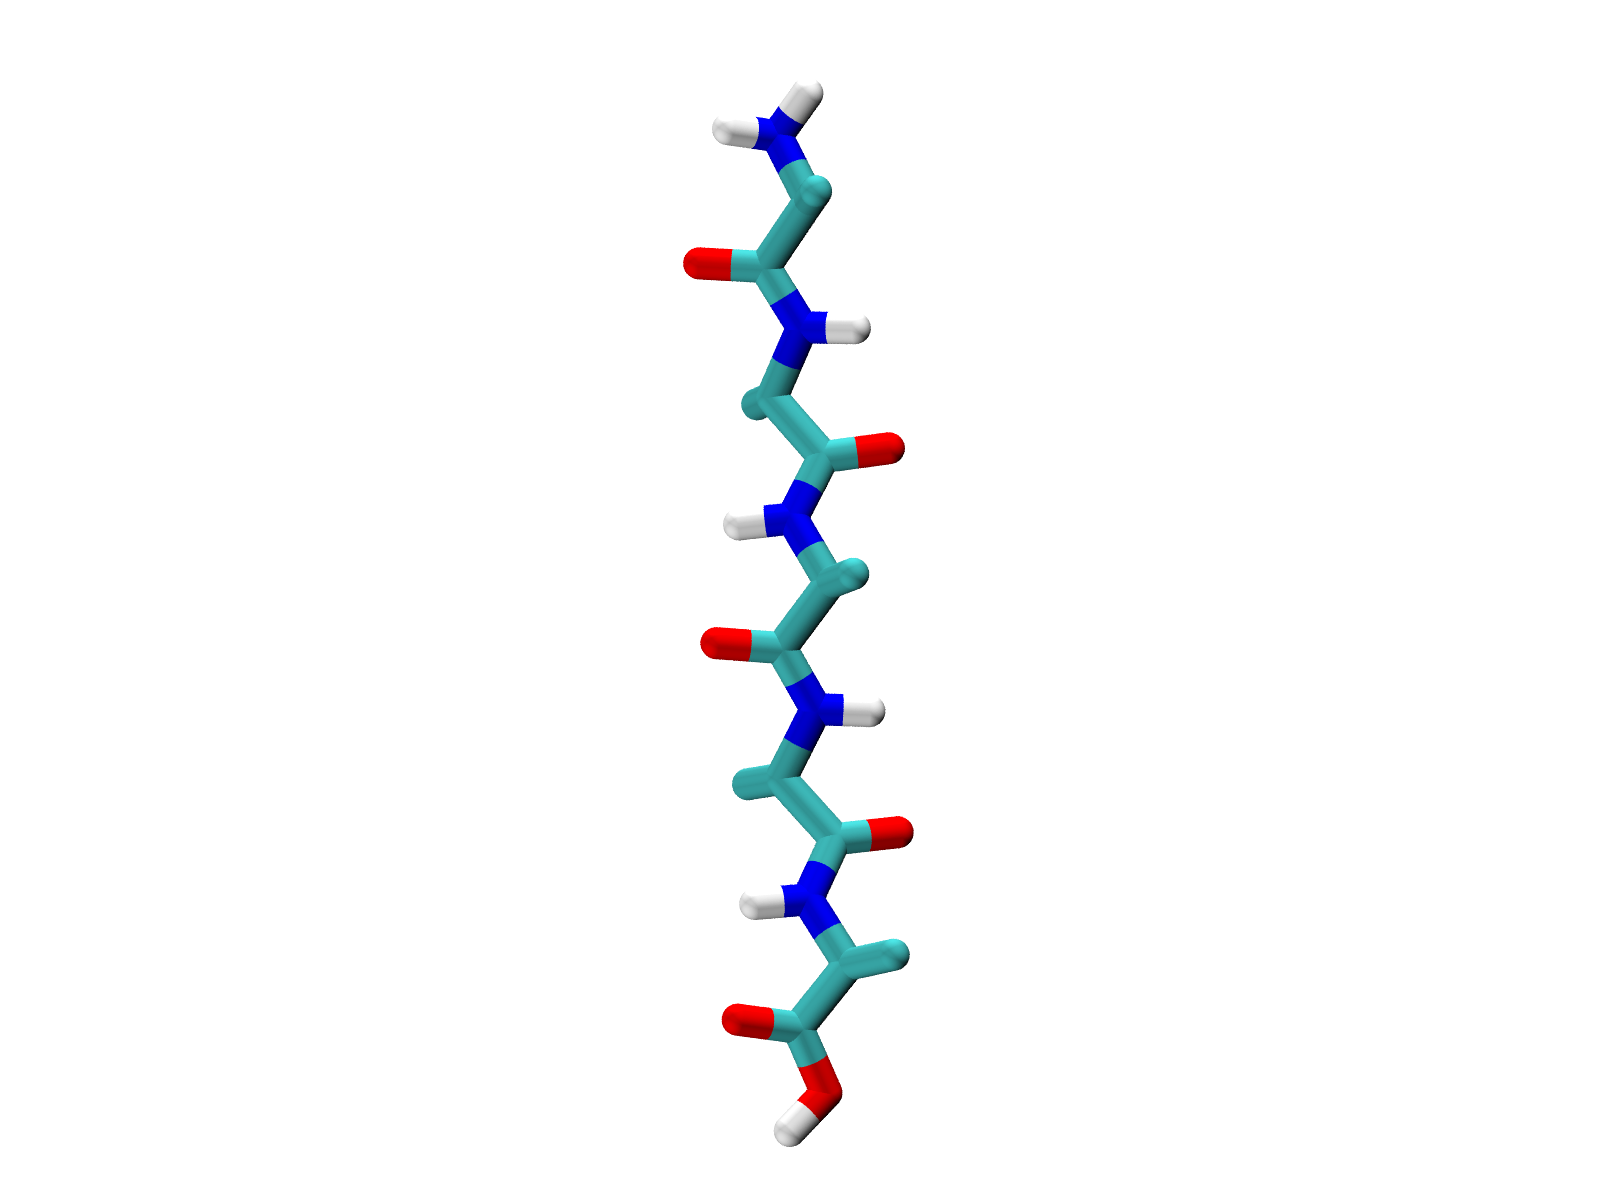
\includegraphics[width=\textwidth]{Figures/Chapter_5/5ALA_extended.png}
    \caption{Representation of extended-($ALA_5$) configuration.}
    \label{fig:5ALAext}
    \end{subfigure}
    
    \caption{Graphic representation of both penta-Alanines (helix and extended) configurations generated with VMD.}
    \label{fig:5_ALA_struct}
\end{figure}


\subsection{About GROMOS software}\label{subsec:about_}
GROMOS is an acronym of the \textbf{GROningen MOlecular Simulation} computer program. It's a software package used for computer simulations of molecular systems like proteins, inorganic and organic chemical compounds, DNA, etc, developed since 1978 and it is written in C++ programming language.
In order to preform MD simulations with GROMOS software, three main elements must be generated and used in every step of the simulation. They are:
\begin{itemize}
    \item Topology of the system (\textbf{*.top} file)
    \item Spacial coordinates of the system (\textbf{*.cnf} file)
    \item Input file (\textbf{*.imd} file) with the parameters for the MD simulation
\end{itemize}

\subsubsection{Building a topology}
The first task is to generate a molecular topology file containing the topological and force-field data concerning the molecular system under consideration. The topology information is referred to the data on the covalent structure, atomic masses, charges, van der Waals parameters, atom-atom distance restraints specification, restraints specification, local-elevation dihedral angles specification, etc. Every constant and parameter described in section \ref{subsec:FF} it's contained in the \textbf{*.top} file. In GROMOS, a molecular topology is generated from molecular topology building blocks which carry the topological information of molecules like amino acid residues, nucleotides, etc. The molecular topology
building blocks can be linked together into a complete molecular topology file using the GROMOS++ program \texttt{make\_top}. In this work, the \textbf{GROMOS-54a7} force-field was selected to preform the molecular dynamics simulations. 

\subsubsection{Generating atomic cartesian coordinates}
The next step is to generate the configurational information regarding to the atomic coordinates and atomic coordinate dependent or related quantities, such as velocities and forces, atom-atom distances, dihedral angles, energies, size of the computational box, etc. These two types of information (topologycal and configurational) are generally stored in separate files, since configurations change continuously during a simulation, whereas molecular topological data generally do not change.

Coordinates for biomolecules are often available from X-ray or Nuclear magnetic resonance spectroscopy (NMR) experiments and can be obtained in Protein Data Bank (PDB) format, which can be converted to GROMOS format using the GROMOS++ program \texttt{pdb2g96}. In this case, the \textbf{*.pdb} files for both alanines configurations (extended and helix) are generated using VMD's plugin \texttt{Molefacture} which is a user interface to create and edit molecules. This includes the ability to add, delete, or manipulate their structure at an atomic level, and to build new components from a library of common fragments.
As the coordinates for hydrogen atoms are not present in \textbf{*.pdb} files (usually) they have to be generated using the GROMOS++ program \texttt{gch}. In the standard GROMOS force fields, part of the hydrogen atoms (polar, aromatic) are explicitly treated, whereas other hydrogen atoms (aliphatic, some aromatic) are implicitly treated by incorporation into the (carbon)atom to which they are attached. Program \texttt{gch} calculates optimal positions for hydrogen main structure atoms.

\subsubsection{Energy minimisation of the peptide}
Before putting any peptide into a box of solvent, its configuration has to be relaxed by energy minimisation. The use of this technique with an empirical energy function such as Equation \ref{eq:v_general} is a widely used tool for obtaining low-energy configurations of a molecular system. In this work, the \textit{steepest descent method} is implemented for this propose \cite{van1988role}.
When applying energy minimization algorithms one searches for a minimum energy configuration of a system by moving (approximately) along the direction of the gradient of the potential energy through configuration space.
\begin{equation}
    \Delta r_i \sim -\frac{\delta }{\delta r_i}V(r_1,r_2,...,r_n)
    \label{eq:gradient}
\end{equation}
where $\Delta r_i$ is the change in position, $V$ the potential energy function given by Equation \ref{eq:v_general}, and $r_i$ the position vector of a particle $i$. 

Since all configurations used for simulations were not directly obtained from physical data, but instead generated with VMD, these artificial structures can possess high amounts of potential energy so they were minimized with a maximum minimization time of 5 [$ps$] in 2 [$fs$] steps (maximum time because the simulation also stops if the potential energy difference between two steps is less than a certain minimum, in this case 0.1 [$kJ/mol$])

\subsubsection{Solvating the peptide}\label{subsubsec:sim_box}
Once the structure is minimized, the next step is to put the peptide in a box of solvent using the GROMOS program \texttt{sim\_box} which can solvate the solute in a pre-equilibrated box of solvent molecules. There are three types of box's shapes (rectangular, truncated octahedron and cilindrical), and a water model must be determined. In this work, the rectangular box shape and a SCP-water model was selected to perform the simulations. 

In order to relax the unfavorable atom-atom contacts between the solute and the solvent, energy minimisation of the solvent should be performed while keeping the solute positionally restrained (i.e. connecting the atom to a reference position by a spring). The restraining is achieved by a harmonic force term with a force constant determined in the simulation input file (\textbf{*.imd}). 
\begin{figure}[h]
    \centering
    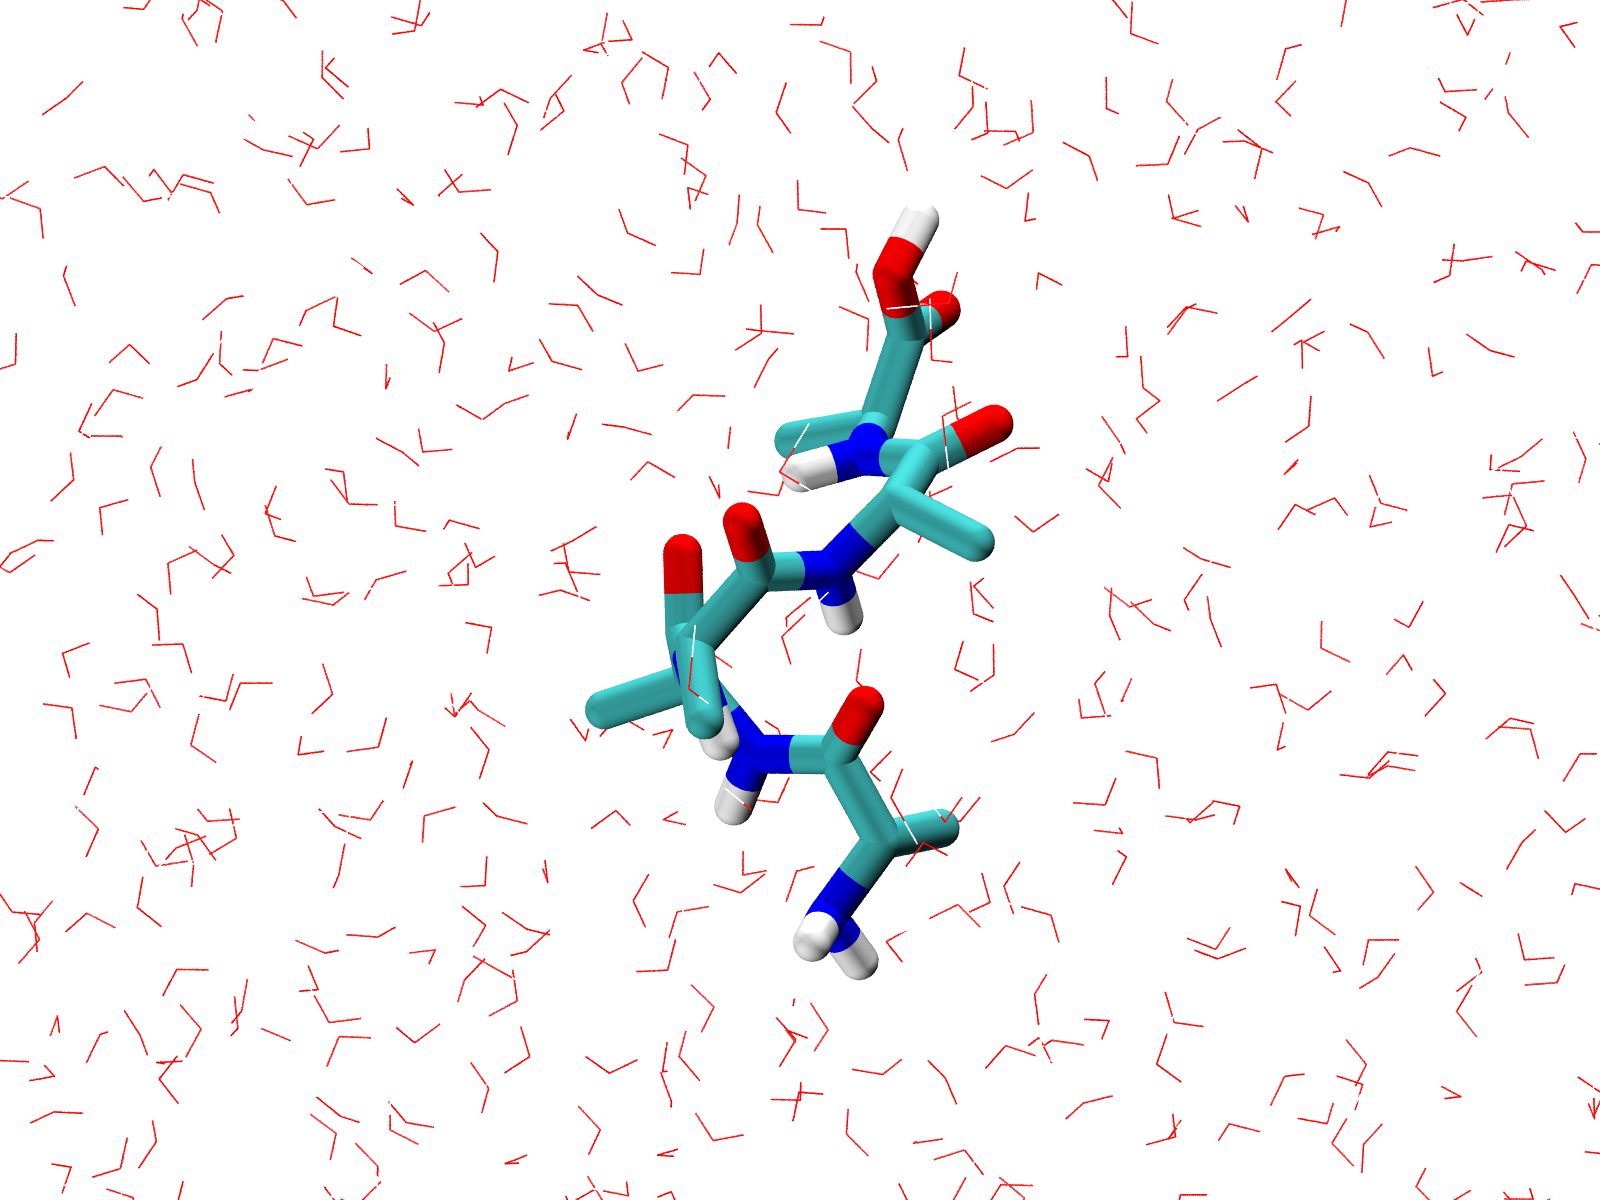
\includegraphics[scale=0.18]{Figures/Chapter_5/sim_box.png}
    \caption{Penta-alanine in box full of water molecules.}
    \label{fig:sim_box}
\end{figure}

\begin{table}[th] %th for exact position.
    \centering
    \begin{tabular}{c|cc|cc}
    \toprule
    \multirow{2}{4em}{n-ALA}           &   \multicolumn{2}{c|}{\textbf{Helix}} & \multicolumn{2}{c}{\textbf{Extended}}\\

    &   Box size $[nm^3]$ & $N^o$ atoms    &   Box size $[nm^3]$     &   $N^o$ atoms\\
    \midrule
    1         &   2.879  &   2310                  &   2.921                  &   2421\\
    2         &   3.136  &   2985                  &   3.067                   &   2814\\
    3         &   3.166  &   3078                  &   3.028                  &   2706\\
    4         &   3.075  &   2820                  &   3.183                  &   3138\\
    5         &   3.148  &   3000                  &   3.545                   &   4386\\
    6         &   3.119  &   2937                  &   3.901                   &   5820\\
    7         &   3.299  &   3.119                  &   4.263                   &   7551\\
    8         &   3.568  &   4443                  &   4.620                   &   9537\\
    9         &   3.736  &   5106                  &   4.981                  &   12099\\
    10         &   3.511  &   4260                  &   5.269                   &   14202\\
    \bottomrule
    \end{tabular}
    \caption{Summarize of the 20 system's dimensions and the number of atoms to be simulated.}
    \label{table:box_size}
\end{table}     

At this point, two \textbf{energy groups} are defined: One is the solute and the other the solvent. If one want to add, for example, counter ions to the simulation, it will be helpful to assign them other groups number. This is a key component because later, for the energy analysis, one can preform individual analysis between energy groups. 

\subsubsection{Thermalization and equilibration}

After generated the topology and initial coordinates for the system, the next step is to generate initial velocities. Since not all molecules from the system travel at the same speed, initial velocities can be randomly generated from a Maxwell-Boltzmann distribution at a low temperature and the system is slowly heated up to the final production simulation temperature:
\begin{equation}
    f(v)=\left ( {\frac{2}{\pi}}\right )^{1/2} \left ( \frac{m}{kT}\right )^{3/2} v^2exp\left [ -\frac{mv^2}{2kT} \right ]
    \label{eq:thermalization}
\end{equation}
were $f(v)$ is the probability distribution of the velocity $(v)$ for a particle of mass $m$ and $kT$ is the product of Boltzmann’s constant and the thermodynamic temperature \cite{muller2013basics}.

The atoms of the solute are positionally restrained and these restraints are loosened while heating up. With the help of these restraints you make sure that the random initial velocities do not disrupt the initial conformation too much. In this work, the equilibration process of every peptide was divided in 5 steps, ranging from 60 [K] to 298.15 [K]. In every step, the temperature of both, peptide and solvent, were increased by 60 [K] in a simulation window of 100 [ps]. Figure \ref{fig:totkin} shows the result of the process. 

\begin{figure}[h]
    \centering
    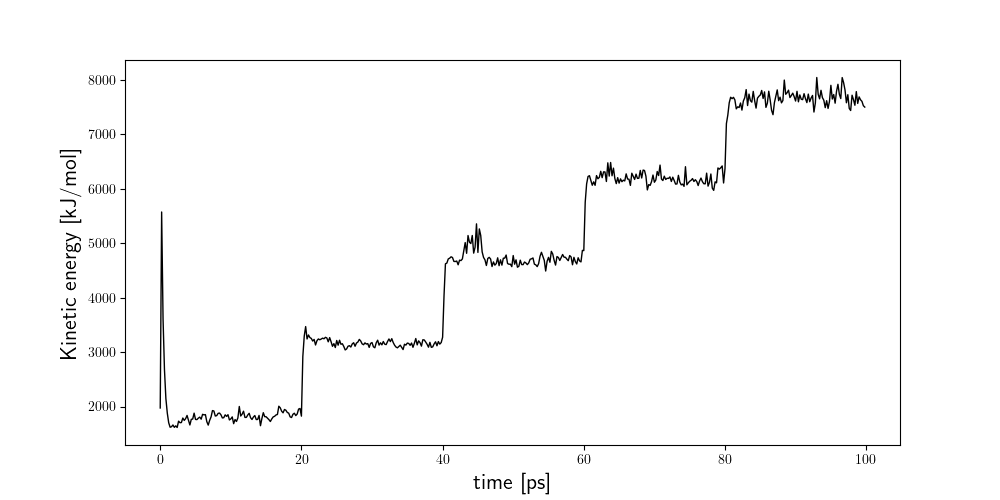
\includegraphics[scale=0.65]{Figures/Chapter_5/totkin.png}
    \caption{The kinetic energy during the equilibration process of the helix penta-alanine.}
    \label{fig:totkin}
\end{figure}





\subsection{Molecular Dynamics Simulation}\label{subsec:MDS}
The equilibration period already produced a short simulation at constant temperature and volume. At this point we want to elongate the simulation to any time window defined by the user, under constant temperature and pressure.

All MD simulations run for this work had a total length of 100 $[ns]$ with a timestep of 2 $[fs]$ using the leapfrog algorithm described in Section \ref{subsubsec:leapfrog}. The SHAKE algorithm \cite{ryckaert1977numerical} was employed to constrain all bonds to their reference values with a relative tolerance of $10^5 [kJ/mol-nm^{2}]$. In order to study only the effects of generating the dry cavity, the solute must be \textbf{positionally restrain} using the same method, to minimizes the changes in entropy related to configurations that can generates the movement of the peptide across the water box. This is accomplished by generated two extra configuration files, in which the positionally restrained (\textbf{*.pos}) atoms and the reference coordinates(\textbf{*.rpr}) are specified, and are generated from the origin coordinate file (\textbf{*.cnf}).

Periodic boundary conditions with a cubic box were applied according to the information provided in Table \ref{table:box_size}.
Non-bonded interactions were computed using a triple range cut-off. Interactions within a short-range cut-off of $0.8 nm$ were computed every time-step, from a pair-list that was generated every 5 steps. At these time points, interactions between $0.8$ and $1.4 nm$ were also computed which were kept constant between these updates. A reaction-field contribution was added to electrostatic interactions approximating for a homogeneous medium outside the $1.4 nm$ cut-off, employing the relative permittivity of SPC water ($\epsilon_w=61$) \cite{tironi1995generalized}. Finally, all simulations were simulated using the isobaric isothermic ensemble (NPT) using the weak-coupling (Berendsen thermostat and barostat) scheme for temperature ($298.15 [K]$) and pressure ($1 [atm]$) control \cite{berendsen1984molecular}. 


\subsection{Free Energy Calculations}

As it is mentioned in Section \ref{subsec:TI}, The free energy difference ($\Delta G$) between two states A and B, can be calculated using Equation \ref{eq:TI}. This equation includes all the potential interactions present in the system. In this case, there are two sources of energy interactions: peptide-peptide (P-P), peptide-solvent (P-S) and solvent-solvent (S-S) interactions. (Notice that the coulomb interactions does not contribute to the Hamiltonian because each atom's charge present in the peptide, were set to 0). 
\begin{equation}
    \left \langle \frac{\partial H}{\partial\lambda} \right \rangle^{vdw}_{\lambda} = \left \langle \frac{\partial H}{\partial\lambda} \right \rangle^{vdw}_{P-P} + \left \langle \frac{\partial H}{\partial\lambda} \right \rangle^{vdw}_{P-S}.
    \label{eq:dHdl_pp}
\end{equation}
Both terms in Equation \ref{eq:dHdl_pp} contributes to the total numerical result of the free energy change between the states A and B, but, the main objective of this work is to calculate only the \textbf{free energy of forming the dry cavity} generated by the non-polar interaction ($\Delta G^{vdw}$) of the solvated solute. Taking this into account, the therm $\left \langle \frac{\partial H}{\partial\lambda} \right \rangle^{vdw}_{P-P}$ does not contribute to generate the cavity because only consider the interaction between it self, so it must be unchanged during the $\lambda$-transition, i.e, the van der Waals \textbf{peptide-peptide} interactions must remain unchanged during the process. 
This was obtain by adding an extra block (\texttt{LAMBDAS}) to the molecular dynamics input file (\textbf{*.imd}) which control the interaction between the coupling parameter $\lambda$, and the groups previously define (Sec. \ref{subsubsec:sim_box}). This allows to determine that the parameter only affects the peptide-solvent interaction, groups (1-2). Figure \ref{fig:StateAB} represent this phenomenon. 

\begin{figure}[h]
    \centering
    \begin{subfigure}[t]{0.45\textwidth}
    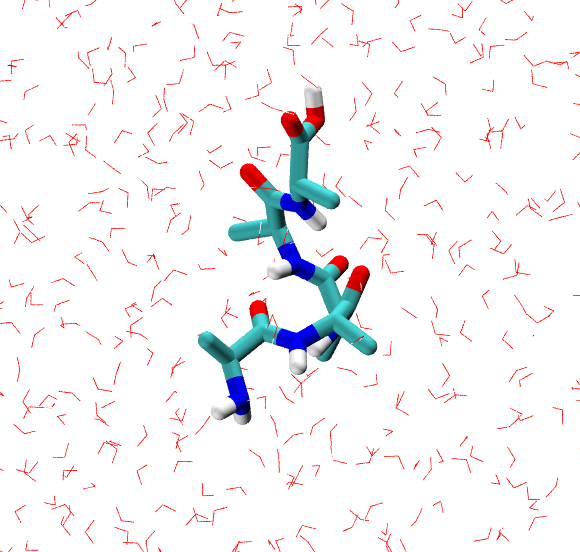
\includegraphics[width=\textwidth]{Figures/Chapter_5/StateA.png}
    \caption{Representation of state \textbf{A}. All van der Waals interactions on.}
    \label{fig:StateA}
    \end{subfigure}
    \hspace{0.5cm}
    \begin{subfigure}[t]{0.45\textwidth}
    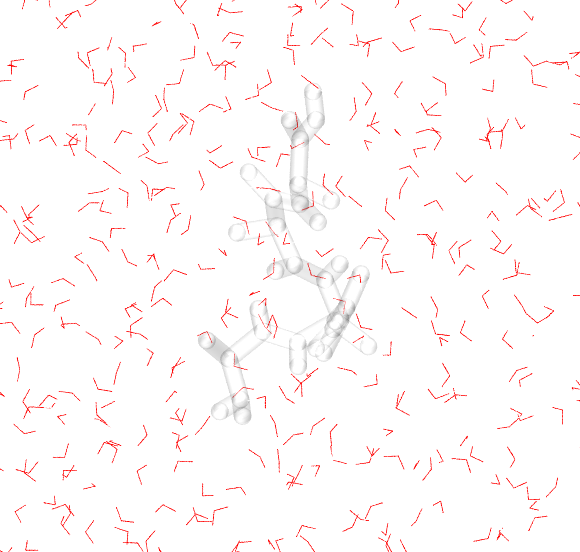
\includegraphics[width=\textwidth]{Figures/Chapter_5/StateB.png}
    \caption{Representation of state \textbf{B} with all van der Waals interactions equal to 0: the ``dummy molecule".}
    \label{fig:StateB}
    \end{subfigure}
    \caption{Graphic representation of the process of \textbf{Thermodynamic Integration} where a molecules is turn into a dummy molecule according to the couple parameter $\lambda$. The transition goes froms State A to State B.}
    \label{fig:StateAB}
\end{figure}

\subsubsection{Thermodynamic Integration's Numerical Error}\label{subsubsec:TIerror1}
To compute the free energy between state A and B, the integrate curve over all $\lambda$-steps must be calculated. For each value of $\lambda$, every $\frac{\partial H}{\partial \lambda}$ in the soft-core potential form (Sec. \ref{subsubsec:softcore}) is computed. To avoid numerical errors related to the smoothness of the curve generated, and further numerical integration, the transition over the $\lambda$-points must assure that the function generated by Equation \ref{eq:TI} is smooth enough to prevent this.
This is accomplish by simulate more $\lambda$-points in between other to generate more $\frac{\partial H}{\partial \lambda}_i$ values for the curve. In this case, five versions of TI were preformed to determine the total number of $\lambda$-steps: $[10,17,20,23,32]$. Al five versions are attached to this work in \ref{subsec:TI_evolve}. As a result of that, the $\lambda$ space, between 0 and 1 were distribute in 32 discrete points: 

\begin{table}[th] %th for exact position.
    \centering
    \begin{tabular}{|c|c|c|c|c|c|c|c|}
    \toprule
         0.000 & 0.400 & 0.600 & 0.690 & 0.715 & 0.735 & 0.800 & 0.880 \\
         0.100 & 0.450 & 0.625 & 0.700 & 0.720 & 0.740 & 0.820 & 0.900 \\
         0.200 & 0.500 & 0.650 & 0.705 & 0.725 & 0.760 & 0.840 & 0.950 \\
         0.300 & 0.550 & 0.675 & 0.710 & 0.730 & 0.780 & 0.860 & 1.000 \\
    \bottomrule
    \end{tabular}
    \caption{Distribution of 32 $\lambda$ points between 0 and 1.}
    \label{table:l_points}
\end{table}

For each window, 0.2 $[ns]$ of equilibration was performed, followed by 15 $[ns]$ of production MD, from which the free energy differences between adjacent $\lambda$ values were computed with the methods outlined above, and the total free energies were calculated by integrate the curve over all the $\lambda$-steps. 

 


\section{Results and Discussion}\label{sec:results}

Here, the results of the free energies of disappear the van der Waals interactions for 20 $n-alanines$ with n ranging from $1$ to $10$, in both configurations (helix and extended) are presented under the methods highlighted above.

\subsection{Energy Interaction Results}

First, the discrete transition between states A and B acopled with the $\lambda$-parameter, explained in Section \ref{subsec:TI} is presented in Figure \ref{fig:peptide_interactions}. 

\begin{figure}[h]
    \centering
    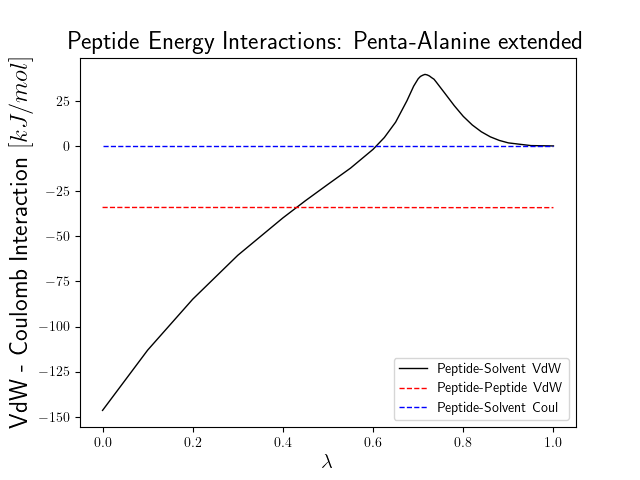
\includegraphics[scale=0.8] {Figures/Chapter_6/Interactions.png}
    \caption{Evolution of interactions between peptide and solvent while the transition of the $\lambda$ parameter.}
    \label{fig:peptide_interactions}
\end{figure}

The energy interactions between the peptide and the solvent is changed, using the soft core potential function (Equation \ref{eq:softcorepot}), from the initial value calculating with the force-fields parameters and the system configuration, to zero. Here, two important points must be notice: (1) the coulombic interactions is equal to zero during all the transition. This is because as it was said before, the atomic charges were manually set to zero (Section \ref{subsec:strucutre_prep}), and (2), the peptide-peptide interaction remains constant during the transition. This two factors, assures that the free energy change $\Delta G$ corresponds to the free energy required to turn-off the van der Waals interactions between the peptide and the solvent, i.e, the free energy of \textbf{generating the dry cavity on the solvent.} 

Figure \ref{fig:peptide_interactions} is a sample of the penta-alanine energy interactions in extended configuration, of all the 20 results. In addition, Figure \ref{fig:solvent_vdw} shows how the solvent van der Waals interactions evolves with itself during the transition of the $\lambda$-parameter.  
\begin{figure}[h]
    \centering
    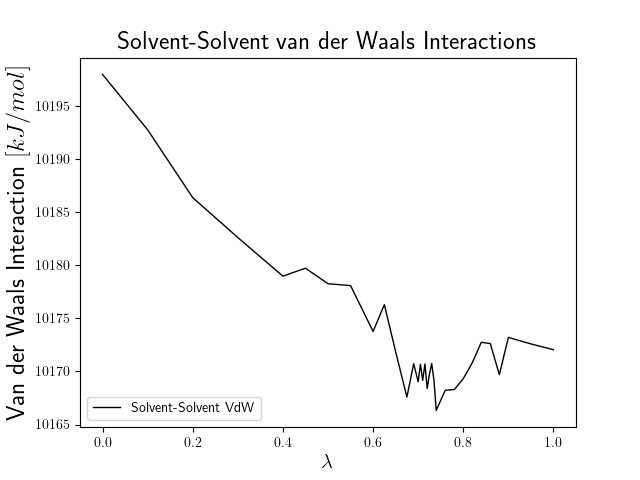
\includegraphics[scale=0.7]{Figures/Chapter_6/Solvent_vdw_Interactions.png}
    \caption{Evolution of van der Waals interactions between the solvent with itself while the transition of the $\lambda$ parameter.}
    \label{fig:solvent_vdw}
\end{figure}

Finally, the coulomb interaction between the solvent is presented in Figure \ref{fig:solvent_coul}. Notice that both interactions becomes more negative, i.e, more favorable during the transition because in the lack of interaction between molecules, or the presence of a dummy atom, allows the connection between more solvent molecules. We can think of this like the normal molecule is acting as a screen for the solvent molecules that are at the other side. in the process of tunr-off the peptide-solvent interactions, one can see how the solvent molecules that wasn't interacting with themselves, starts to contribute to the total value of these interactions. 
\begin{figure}[h]
    \centering
    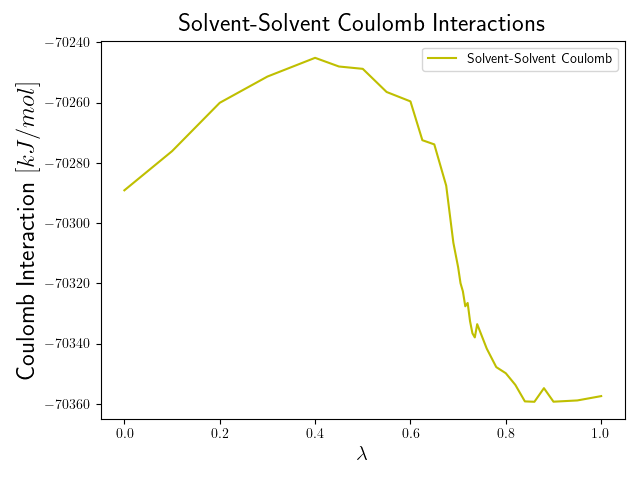
\includegraphics[scale=0.7]{Figures/Chapter_6/Solvent_coul_Interactions.png}
    \caption{Evolution of coulomb interactions between the solvent with itself while the transition of the $\lambda$ parameter.}
    \label{fig:solvent_coul}
\end{figure}

\subsection{Free energy Results}
Figure \ref{fig:TI_7ALA} illustrates the $\frac{\partial H}{\partial \lambda}$ values for each $\lambda$-points define in Section \ref{subsubsec:TIerror1}. This particular result correspond to the hepta-alanine ($ALA_7$) in helix configuration, and the total result of the free energy of solvation correspond to the integrate of all the points over the $\lambda$ space. 
\begin{figure}[h!]
    \centering
    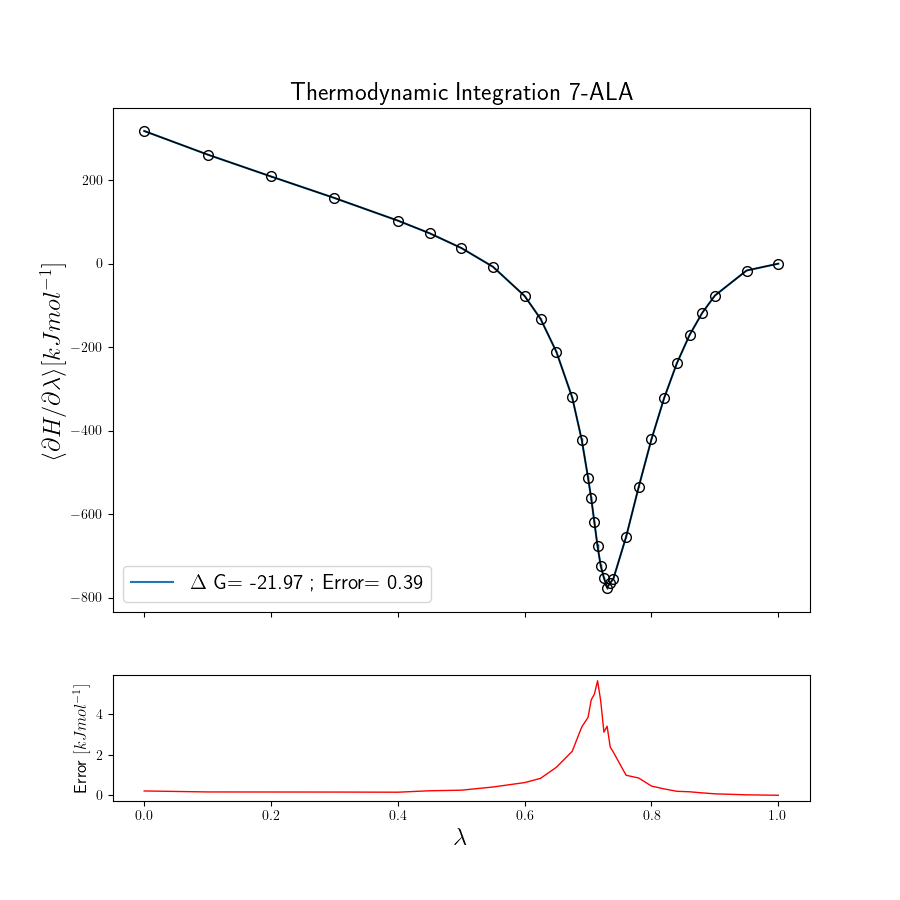
\includegraphics[scale=0.6]{Figures/Chapter_6/TI.png}
    \caption{TI curve for hepta-alanine in helix configuration.}
    \label{fig:TI_7ALA}
\end{figure}
This exercise was preform for every configuration and the results are presented as follows: Table \ref{table:DG_final} summarizes each numerical result for each configuration, both extended and helix, and Figure \ref{fig:DG_total} illustrates the free energies. All TI curves are attached to this work in the Appendix \ref{subsec:TI_curves}.


\begin{table}[th] %th for exact position.
    \centering
    \begin{tabular}{c|cc|cc}
    \toprule
    \multirow{2}{4em}{n-ALA}           &   \multicolumn{2}{c|}{\textbf{Helix}} & \multicolumn{2}{c}{\textbf{Extended}}\\

    &    $\Delta G_{cav}$ $[kJ/mol^{-1}]$ & Error $[kJ/mol^{-1}]$     &  $\Delta G_{cav}$ $[kJ/mol^{-1}]$    &    Error $[kJ/mol^{-1}]$  \\
    \midrule
    1         &   -6.350  &   0.153                  &   -7.752                 &   0.152\\
    2         &   -10.198  &   0.207                 &   -10.488                &   0.213\\
    3         &   -12.709  &   0.261                 &   -12.641                &   0.242\\
    4         &   -16.198  &   0.291                 &   -14.020                &   0.291\\
    5         &   -16.524  &   0.333                 &   -15.767                &   0.323\\
    6         &   -20.223  &   0.361                 &   -18.007                &   0.356\\
    7         &  -21.969  &   0.391                  &   -19.996                &   0.376\\
    8         &   -23.102  &   0.422                 &   -21.915                &   0.383\\
    9         &  -24.663  &   0.433                  &   -24.103                &   0.420\\
    10        &   -26.584  &   0.460                 &   -25.523                &   0.477\\
    \bottomrule
    \end{tabular}
    \caption{Summarize of the 20 free energies calculations with statistical error.}
    \label{table:DG_final}
\end{table}

\begin{figure}[h!]
    \centering
    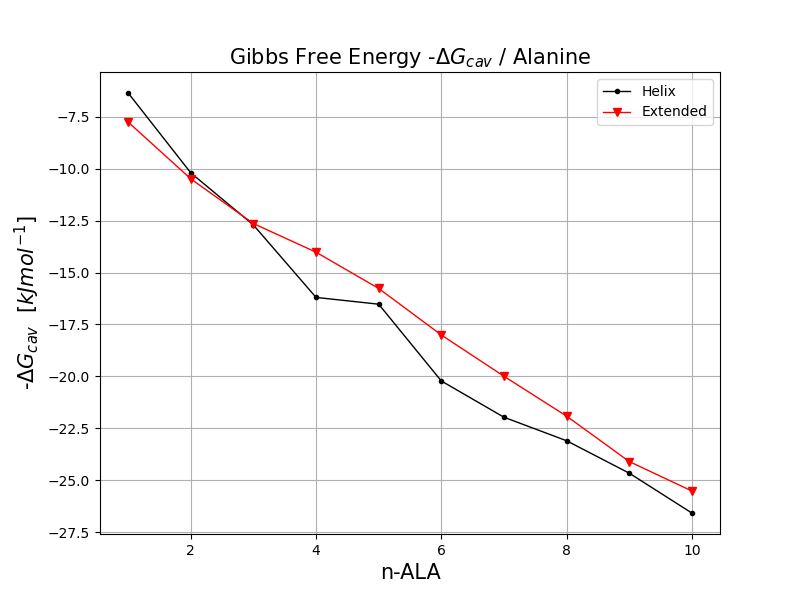
\includegraphics[scale=0.6]{Figures/Chapter_6/results_1.png}
    \caption{Solvation free energies of the extended and helix alanine peptides plotted as functions of the number (N) of residues in the peptide.}
    \label{fig:DG_total}
\end{figure}

As it it seen in Figure \ref{fig:DG_total}, a clear linear relationship between the size of the peptide that it is solvated, and the free energy required to generate the cavity it's seen. 

\subsubsection{Statistical Error}
As it is seen in Figure \ref{fig:TI_7ALA}, there are error values related to each $\lambda$-point. One can think that as a simulation is preform, there is no experimental measure to compare the results to estimate an error.
For this, GROMOS software calculate \textbf{averages} and \textbf{standard deviation} by blocks for to determine a \textit{statistical error} to each result. This is: all teh simulation samples are group in several blocks and for each block, the mean of the propertie of interest, is calculated. Then the mean of the mean of the blocks is reported and the standard deviation of this mean. This is because what we measure in general behaves like normal distributions, so the deviation does not tell us the error, but tells us other properties. But if we make blocks we can estimate as if we had made independent measurements, and from each one we have taken a single value (the average). Whit this, it's possible to report an error \cite{allen2017computer}. 

To estimate the precision of Equation \ref{eq:TI}, the following formula can be used for the standard deviation on the mean \cite{daura1996free}:
\begin{equation}
    \sigma\left ( \left \langle \frac{\partial H(\lambda )}{\partial \lambda } \right \rangle_{\lambda_n} \right ) = \left( \frac{S_{\lambda_n}}{N_{conf}} \right )^\frac{1}{2}\sigma\left (\frac{\partial H}{\partial \lambda}\right )
\end{equation}
where $N_{conf}$ denotes the number of configurations over which the ensemble average at $\lambda=\lambda_n$ is taken, and $\sigma\left (\frac{\partial H}{\partial \lambda}\right )$ is calculated as the square root of the variance over the ensemble.
\begin{equation}
    \sigma^2\left (\frac{\partial H}{\partial \lambda}\right )=\frac{1}{N_{conf}}\sum^{N_{conf}}_{t=1} \left[ \frac{\partial H}{\partial \lambda} - \left\langle\frac{\partial H}{\partial \lambda} \right \rangle_{\lambda_n,N_{conf}}\right ]^2
    \label{eq:statistical}
\end{equation}


To calculate the statistical inefficiency, $S_\lambda_n$, the total simulation time at $\lambda=\lambda_n$ is divided into $M$ blocks of length $b$, and $N_b$ configurations are taken from each block such that $M\cdot N_b=N_{conf}$ \cite{allen2017computer}. The variance of the mean is then calculated for each possible block length $b$ as: 
\begin{equation}
     \sigma^2\left ( \left \langle \frac{\partial H(\lambda )}{\partial \lambda } \right \rangle_{\lambda_n,b} \right ) = \frac{1}{M}\sum^M_{m=1}\left[ \left\langle\frac{\partial H}{\partial \lambda}\right\rangle_{\lambda_n,N_b,m}- \left\langle\frac{\partial H}{\partial \lambda} \right \rangle_{\lambda_n,N_{conf}}\right ]^2
\end{equation}
where $\left\rangle ... \right\rangle_{\lambda_n,N_b,m}$ denotes the ensemble average at $\lambda = \lambda_n$ over $N_b$ configurations of the $m-th$ block. $S_\lambda_n$ is then calculated as: 

\begin{equation}
    S_\lambda_n=\lim_{N_b\rightarrow \infty }\frac{N_b \sigma^2\left ( \left \langle \frac{\partial H(\lambda )}{\partial \lambda } \right \rangle_{\lambda_n,b} \right )}{ \sigma^2\left (\frac{\partial H}{\partial \lambda}\right )}
\end{equation}
\par
It is the limiting ratio of the observed variance of an average to the limit expected on the
assumption of uncorrelated Gaussian statistics. Having estimated $S_\lambda_n$, we can write Equation \ref{eq:statistical}. This statistical error is presented in Table \ref{table:DG_final} and in the bottom graph in Figure \ref{fig:TI_7ALA}. This error is corrected by extending the simulation time for the TI because it generates more configuration to sample. This is the main reason why in Section \ref{subsec:MDS} the simulation time for the TI was determined at $15 [ns]$. 

\subsection{Comparison Between Models}\label{subsec:comparison}
For the standard SASA model, described in Equation \ref{eq:G_solv}, $\Delta G_{cav}$ is computed with $\gamma = 2.51 [kJ/mol/nm^2]$ or $0.06 [kcal/mol/\AA^2]$ and $b = -12.55 [kJ/mol]$ or $-3 [kcal/mol]$. For the propose implicit solvent model, the following constants were used according to Equation \ref{eq:CC_implicit}: $\Phi_{static} = 10.7 [kcal/mol/e]$, $\epsilon_{shell} = 7.75$, and $\rho_{shell}=1.8\rho_w$, with $\rho_w=0.0336 \AA^{-3}$ the bulk water density. All this parameters were selected to calibrate the model after compared the results with the Mobley's explicit-solvent free energy perturtabtion (FEP) calculations \cite{mobley2009small}. Figures \ref{fig:helix_comparison} and \ref{fig:ext_comparison} shows these results. 

\begin{figure}[h]
    \centering
    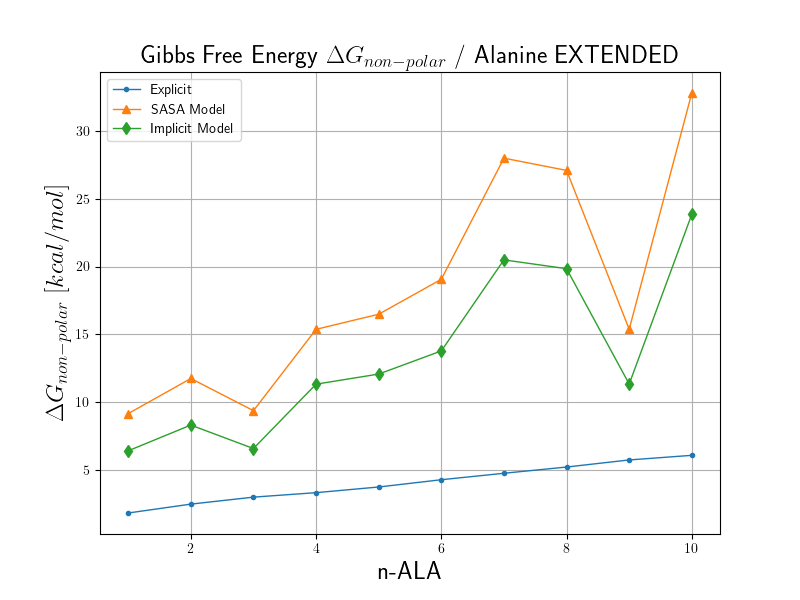
\includegraphics[scale=0.65]{Figures/Chapter_6/comparison_extended.png}
    \caption{Gibbs free energy results from the three models described in this work for extended configuration, per alanine peptide.}
    \label{fig:ext_comparison}
\end{figure}

\begin{figure}[h]
    \centering
    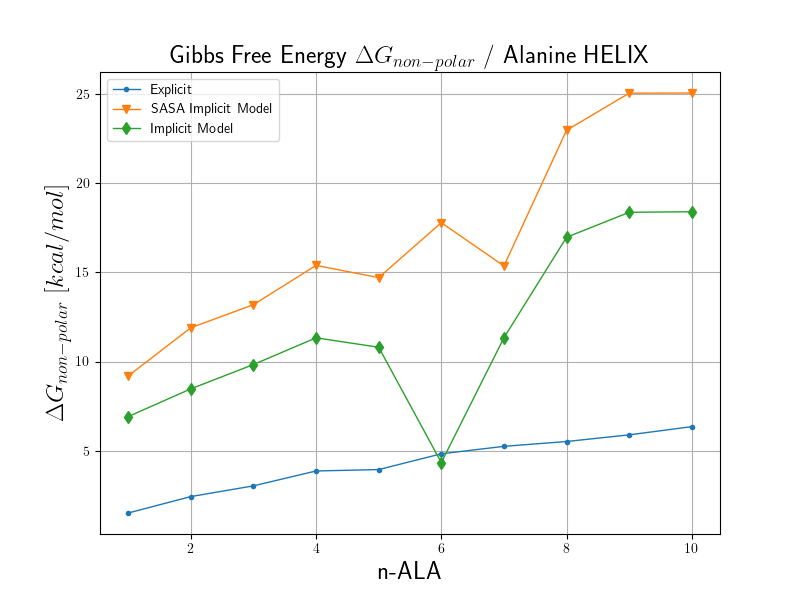
\includegraphics[scale=0.65]{Figures/Chapter_6/comparison_helix.png}
    \caption{Gibbs free energy results from the three models described in this work for helix configuration, per alanine peptide.}
    \label{fig:helix_comparison}
\end{figure}


The use of parametrizations, like the constants described in Section \ref{subsec:comparison}, or the force-field use for the simulations, implies an intrinsic source of uncertainty specially because the lac of empirical measurements related to the free energy calculations. 

As it's seen in Equation \ref{eq:G_solv} and \ref{eq:CC_implicit}, both models depends strongly on the SASA parameter. The standard SASA model can be interpreted as a linear correlation dependent on the SASA factor, and the Implicit solvent model, uses this surface to integrate the potential on it (Eq. \ref{eq:int_shell}). Depending on the method used to generate the SASA factor, both models can carry inaccuracies on the calculations. Figure \ref{fig:SASA_comparison} present the results of tho methods to obtain the SASA factor, one with GROMOS program \texttt{sasa} and the other generated with \texttt{msms} and used in the implicit model.

\begin{figure}[h]
    \centering
    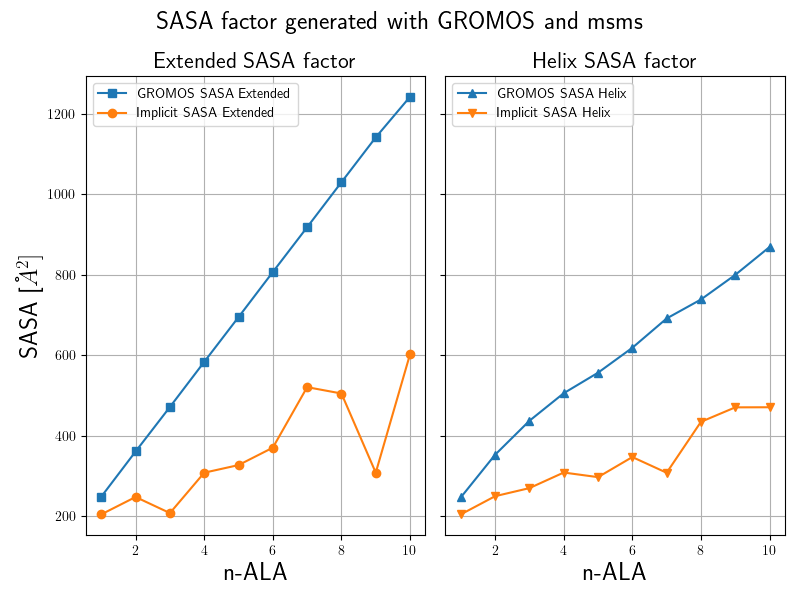
\includegraphics[scale=0.6]{Figures/Chapter_6/SASA_factor.png}
    \caption{Differences between SASA factor generated with \texttt{GROMOS} software and \texttt{msms} program.}
    \label{fig:SASA_comparison}
\end{figure}

The calculation with implicit and standard sasa model (Figure \ref{fig:helix_comparison} and \ref{fig:ext_comparison}), shows ``anomalies" in the free energy values in ($ALA_{9}-extended$) and 
($ALA_{6}-helix, ALA_{7}-helix$). This is correlated with the same behavior in SASA factors showed in Figure \ref{fig:SASA_comparison} which generates the free energy results. To correct this, the method to generate the mesh around the peptide coordinates must be fixed, for example, using a probe with higher molecule radius. 

To measure the accuracy of the prediction for $\Delta G_{np}$ of both models, Pearson coefficient $\rho_p$, root mean square of the difference (RMSD) and the correlation coefficient $R^2$ are used and presented in Table \ref{table:measures_1}. 

\begin{table}[th] %th for exact position.
    \centering
    \begin{tabular}{c|ccc|ccc|c}
    \toprule
    \multirow{2}{4em}{Model}           &   \multicolumn{3}{c|}{\textbf{Helix}} & \multicolumn{3}{c}{\textbf{Extended}}&\textbf{Total}\\

    &   $R^2$ & RMSD   &   $\rho_p $ &  $R^2$ & RMSD   &   $\rho_p $ & \textbf{RMSD}\\
    \midrule
    SASA Model & 0.853 & 22.339 & -0.949 & 0.651 & 24.216 & -0.807 & 23.296\\
    Implicit Model & 0.503 & 16.939 & -0.709 & 0.661 & 18.791 & -0.813 & 17.889\\      
    \bottomrule
    \end{tabular}
    \caption{Comparison of $\Delta G_{np}$ between standard SASA model and the Implicit model proposed.}
    \label{table:measures_1}
\end{table}     

With the parameters described at the beginning of this section, the implicit solvent model presents an improvement of 22.53 \% in predicting the free energy of solvation $\Delta G_{cav}$ over the standard SASA model. 

\subsubsection{Adjust Models constants}

To improve the accuracy of both implicit models, one can adjust the constants to fit the explicit MD curve and improve the overall forecast result. Taking this into account, modifications to both models were made: First, related to the standard SASA model, we propouse the values of $\gamma = 0.025$ and $b = -4.1$ in contrast to the values presented above \cite{cooper2020simple}. Second, we propose a value of $\epsilon_{shell}=3.1$ in contrast to the value reported in \cite{cooper2020simple} of $\epsilon_{shell}=7.75$ as a fitting parameter. The result of this consideration are presented in Figure \ref{fig:new_cc}. Table \ref{table:measures_2} summarizes the results with the new parametrizatrion. 

\begin{figure}[h]
    \centering
    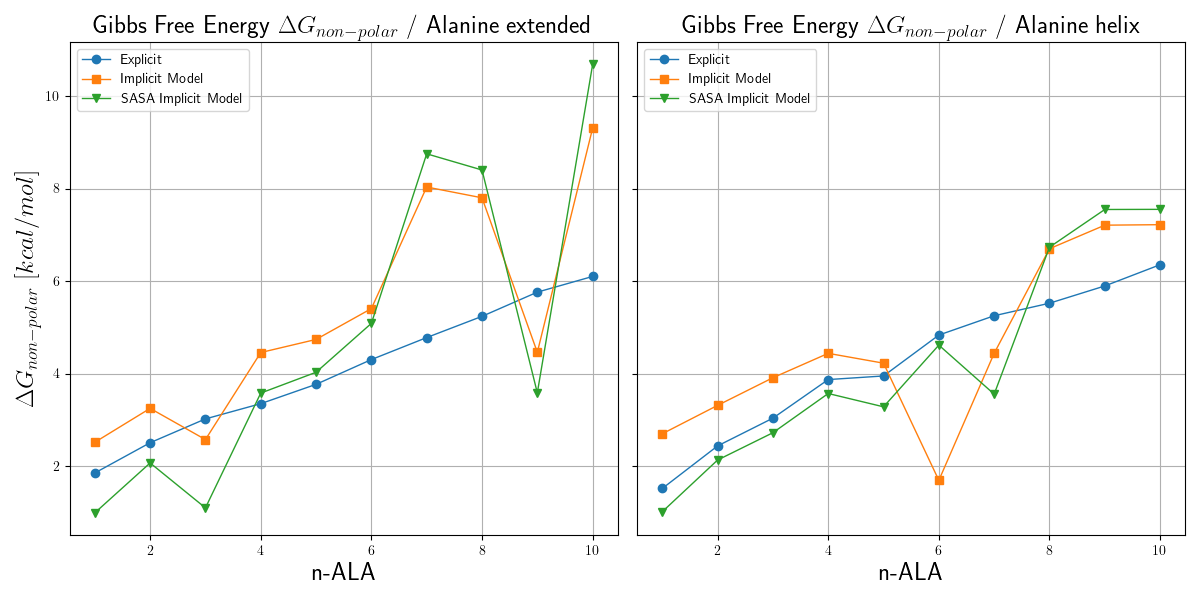
\includegraphics[scale=0.52]{Figures/Chapter_6/New_CC.png}
    \caption{Results after adjustment of parameters $\gamma = 0.025$, $b = -4.1$ for SASA standard model, and $\epsilon_{shell}=3.1$ for the implicit model presented in this work.}
    \label{fig:new_cc}
\end{figure}

\begin{table}[th] %th for exact position.
    \centering
    \begin{tabular}{c|ccc|ccc|c}
    \toprule
    \multirow{2}{4em}{Model}           &   \multicolumn{3}{c|}{\textbf{Helix}} & \multicolumn{3}{c}{\textbf{Extended}}&\textbf{Total}\\

    &   $R^2$ & RMSD   &   $\rho_p $ &  $R^2$ & RMSD   &   $\rho_p $ & \textbf{RMSD}\\
    \midrule
    SASA Model & 0.852 & 9.269 & -0.949 & 0.653 & 9.905 & -0.808 & 9.592\\
    Implicit Model & 0.501 & 9.364 & -0.708 & 0.662 & 9.935 & -0.814 & 9.654\\      
    \bottomrule
    \end{tabular}
    \caption{Comparison of $\Delta G_{np}$ between standard SASA model and the Implicit model with the re-parametrization.}
    \label{table:measures_2}
\end{table}     

\subsection{Conclusions}

In this work, we studied the contribution of van der Waals interactions in the solvation free energy using the Molecular Dynamics (MD) method. This computer simulation methodology allows us to analyze the physical movements of atoms and molecules which are interacting between them for a fixed period of time and used to extract macro-thermodynamic properties like, in this case, free energies. 
The solvation free energy is the energy cost of the process of reorganizing solvent and solute molecules into solvation systems. The solvation process describes the interaction between the solute and solvent molecules and it is govern by electrostatic and van der Waals interactions. In this case, we focus on the free energy which is calculated by the second component. 
To analyze how the property changes with the size of the molecule, 20 alanine-peptide structures were prepared ranging from 1 to 10, and in helix and extended configuration. Finally, free energy results were calculated using the Thermodynamic Integration (TI) method during a MD run. 

From all the 20 TI, it was clear the linear relation between the volume (size) of the alanine peptides, represented in Figure \ref{fig:DG_total}, which is an expected result. If one want to solvate a bigger molecule, higger free energies will result from these solvation processes. In the other hand, as we add identical residues to the next alanine-peptide, from $ALA_1$ to $ALA_2$, from $ALA_2$ to $ALA_3$ and so on, we expect a linear constant characteristic from the alanine peptide. 

We also analyze two implicit methods to estimate this free energy change. One standard method that relates the Solvent-Accessible Surface Area (SASA) with some fitting constants ($\gamma = 0.06 [kcal/mol/\AA^2]$ and $b = -3 [kcal/mol]$) that have shown high accurate results, and a new method that relies in a clearer physical meaning and formulation which uses a capacitor model to emulate the interaction distribution around the solvated peptide. 

To compare the accuracy of the implcit models, the calculations generated with the explicit-MD simulation was used as the ``real/observed" result, and contrast them with the implicit results. It was found the new method for calculating the solvation free energy, and with the parameters described in this work, improves the estimation of the thermodinamic property by \textbf{22.53\%} acording to RMSD parameter. 

It is also proposed a re-parametrization of the fitting constants according to the results presented in this work of $\gamma = 0.025$ and $b = -4.1$ in the case of the standard SASA model, and $\epsilon_{shell}=3.1$ for the propoused implicit solvent model. 




 

\bibliographystyle{ieeetr}
\bibliography{References.bib}

\newgeometry{left=0.4in,right=0.4in,top=0.60in,bottom=0.60in}

\section*{Appendices}
\subsection*{Thermodynamic Evolution}\label{subsec:TI_evolve}

\begin{figure}[h]
    \centering
    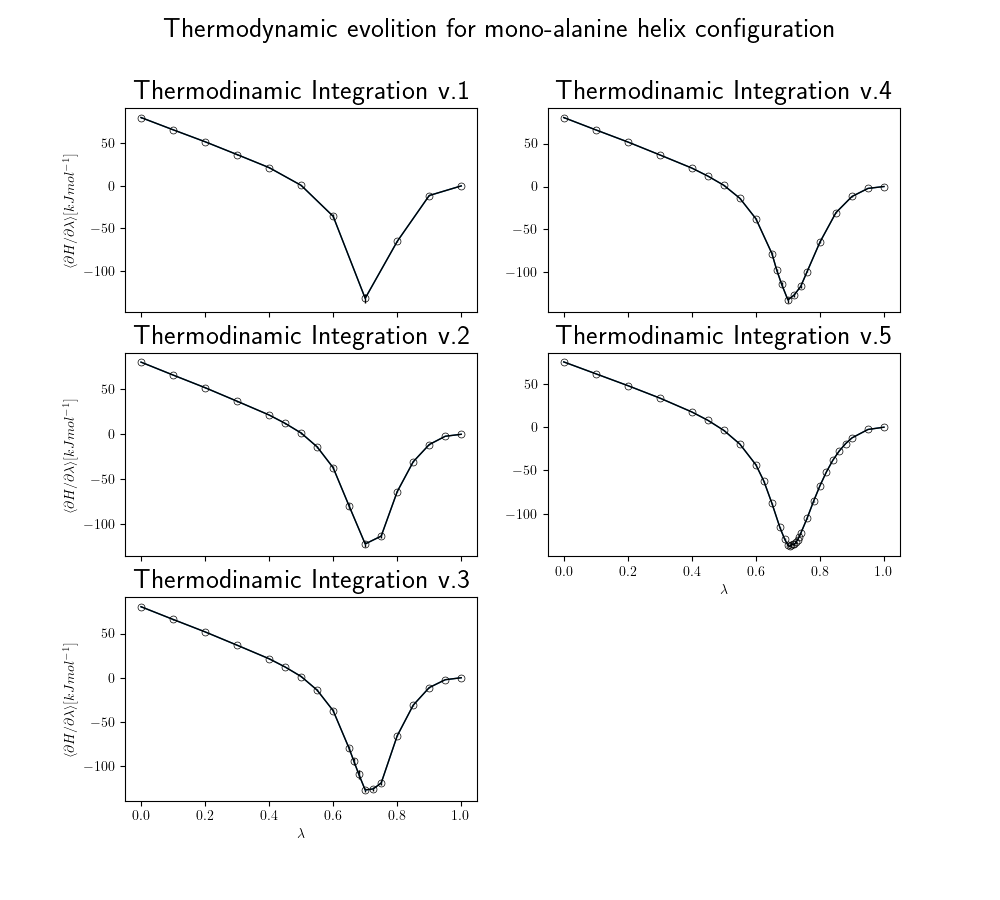
\includegraphics[scale=0.65]{Figures/Chapter_7/TI_evolution.png}
    \label{fig:TI_evolve}
\end{figure}
\newpage

\subsection*{Thermodynamic Integration Curves}\label{subsec:TI_curves}
\begin{figure}[h!]
    \centering
    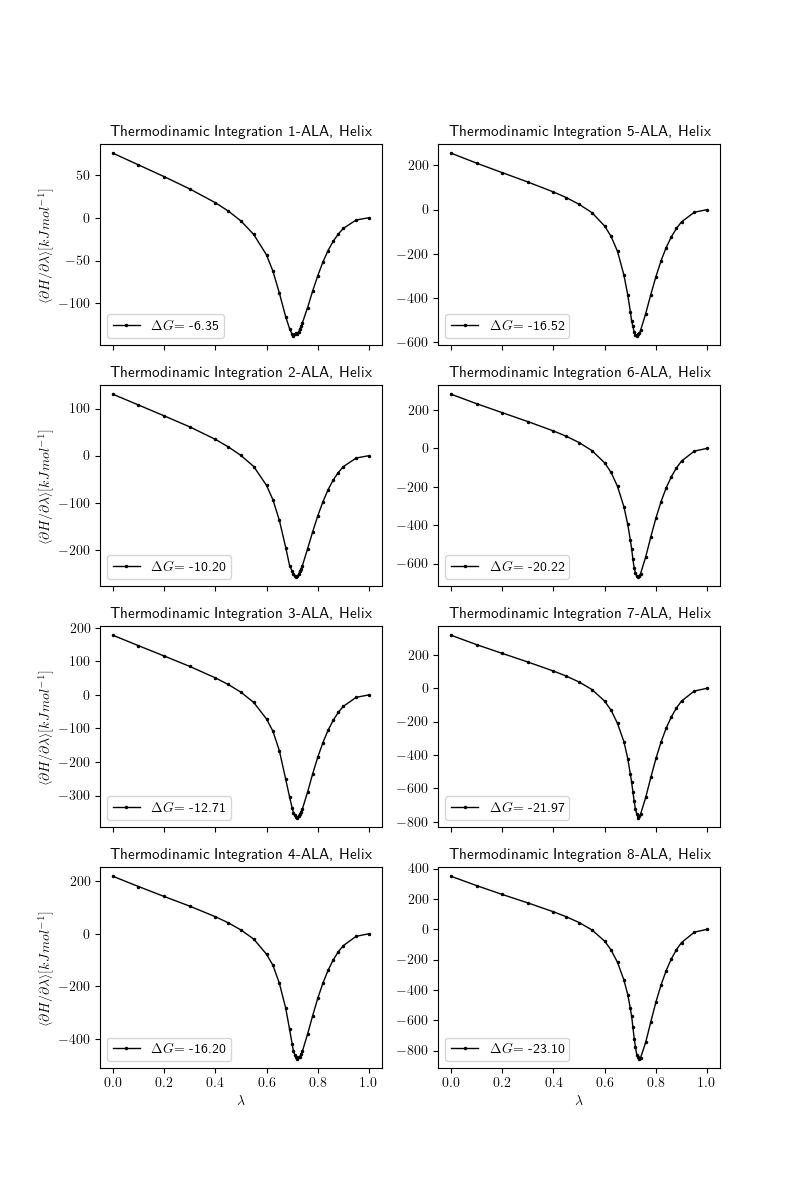
\includegraphics[scale=0.75]{Figures/Chapter_7/TI_curves_1.png}
    \label{fig:my_label}
\end{figure}
\begin{figure}[h]
    \centering
    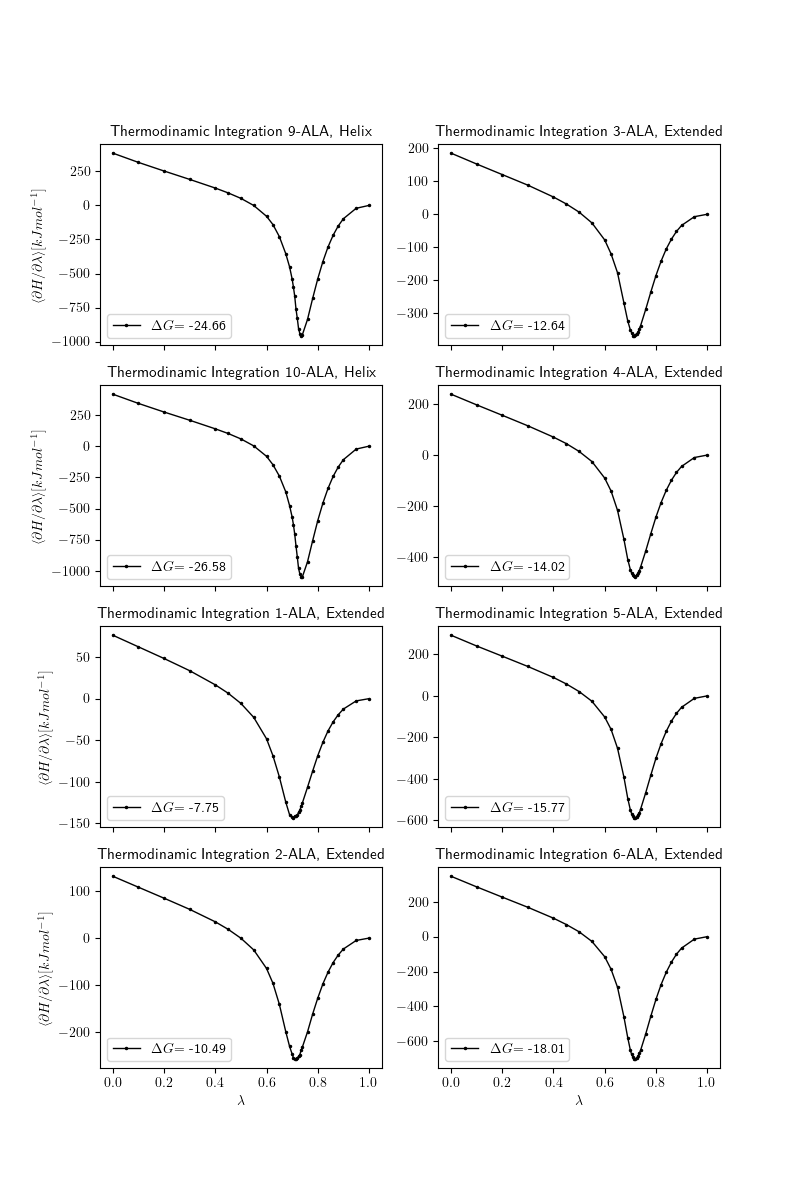
\includegraphics[scale=0.75]{Figures/Chapter_7/TI_curves_2.png}
    \label{fig:my_label}
\end{figure}
\begin{figure}[h]
    \centering
    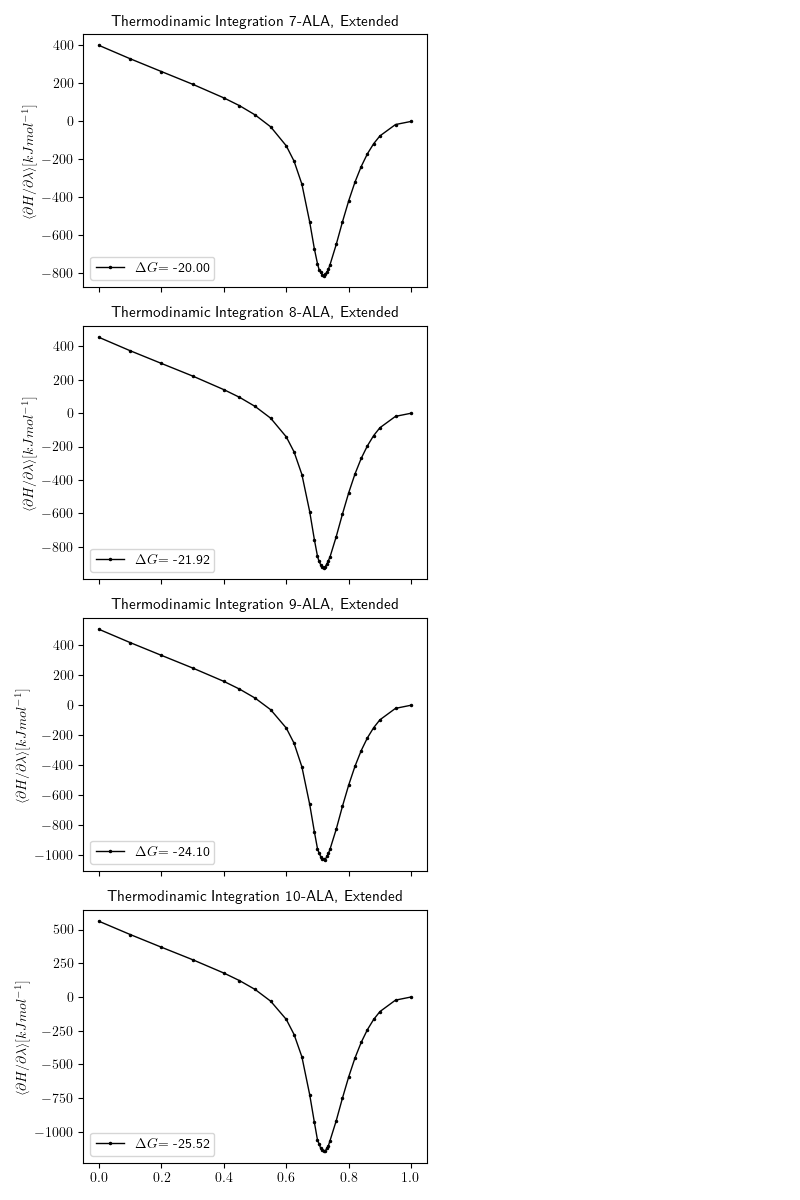
\includegraphics[scale=0.7]{Figures/Chapter_7/TI_curves_3.png}
    \label{fig:my_label}
\end{figure}
\newpage


\end{document}
